\documentclass{report}
\usepackage{hyperref}
\usepackage[ngerman]{babel}
\usepackage{amsmath}
\usepackage{amsfonts}
\usepackage{amsthm}
\usepackage{tcolorbox}
\usepackage[a4paper, total={7in, 9in}]{geometry}
\usepackage[font={scriptsize,it}]{caption}
\usepackage{scrextend}
\usepackage{graphicx}
\usepackage{caption}
\usepackage{subcaption}
\usepackage[utf8]{inputenc}
\usepackage[T1]{fontenc}
\DeclareUnicodeCharacter{2212}{-}
\usepackage{verbatim}
\usepackage{tikz}

\tikzset{
  treenode/.style = {shape=rectangle, rounded corners,
                     draw, align=center,
                     top color=white, bottom color=blue!20},
  root/.style     = {treenode, font=\Large, bottom color=red!30},
  env/.style      = {treenode, font=\ttfamily\normalsize},
  dummy/.style    = {circle,draw}
}

\tikzstyle{level 1}=[level distance=3.5cm, sibling distance=3.5cm]
\tikzstyle{level 2}=[level distance=3.5cm, sibling distance=2cm]

% floating figure for column
\newenvironment{Figure}
	{\par\medskip\noindent\minipage{\linewidth}}
	{\endminipage\par\medskip}

\theoremstyle{definition}
\newtheorem{definition}{Definition}

\theoremstyle{example}
\newtheorem*{example}{Example}

\begin{document}

\begin{titlepage}
   \vspace*{\stretch{1.0}}
   \begin{center}
      \Large\textbf{Advanced Software Engineering 1 - HS20}\\
      \large\textit{Pascal Brunner - brunnpa7}
   \end{center}
   \vspace*{\stretch{2.0}}
\end{titlepage}

% Beispiel Bild
%\begin{Figure}
%   \centering
%    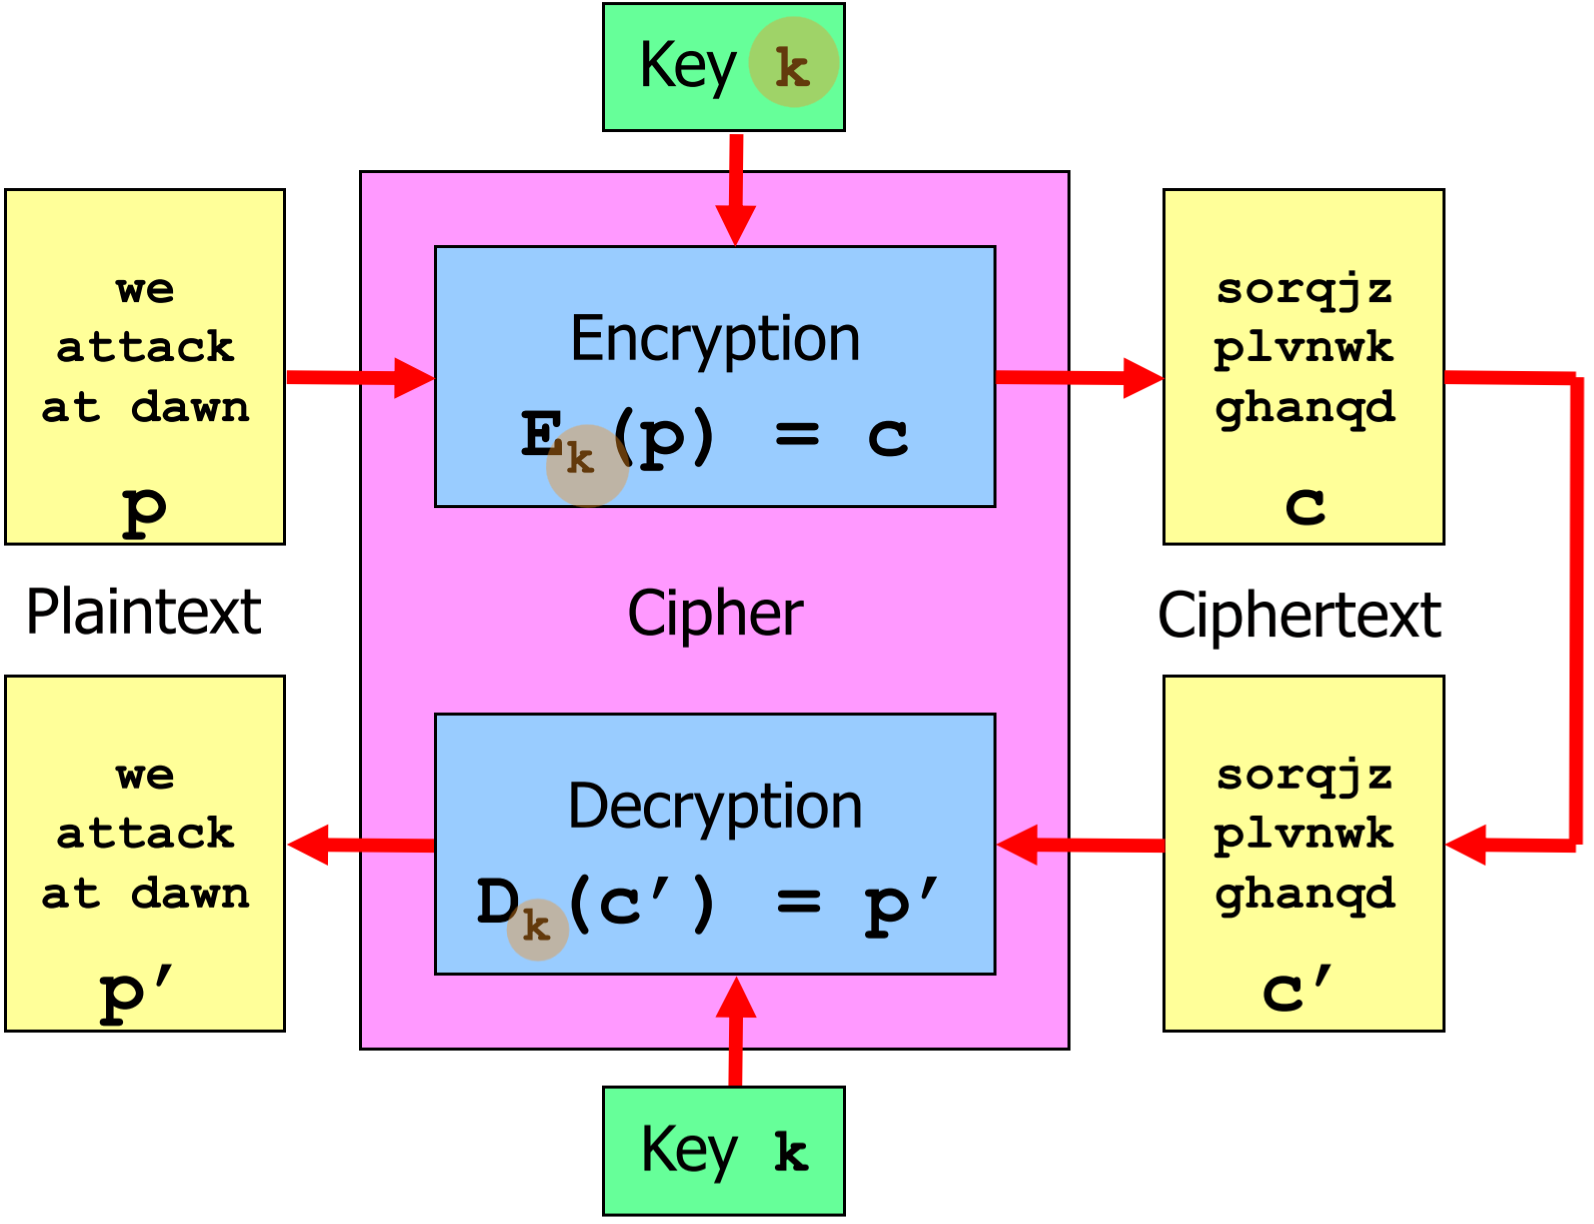
\includegraphics[width=150px]{img/BasicTerminologySecKeyCrypto.png}
%        \captionof{figure}{Basic Terminology basierend auf Secret Key Cryptography}
%        \label{fig:Basic Terminology}
%    \end{Figure}

\tableofcontents

\newpage

\chapter{Einführung ins Software Engineering}

\section{Was ist Software Engineering}
Softwareprodukte sind:
\begin{itemize}
   \item Allgemein: entwickelt für den Verkauf an Anwender
   \item Massgeschneidet: für spezielle Anforderungen / Bedürfnisse
\end{itemize}
Für ein Softwareprodukt gibt es einige Aspekte die dazugehören:
\begin{itemize}
   \item Entwurfsdokumentation
   \item Lastenhaft
   \item Systemprototypen
   \item Systementwurf
   \item Testumgebung $\rightarrow$ rund 50 \% des Aufwandes fällt ins Testing
   \item Konfigurationsmanagement
   \item Systembeschreibung
   \item Produktsupport
   \item Bedienungshandbücher
\end{itemize}

Software ist gemäss IEEE 610.12 wie folgt definiert: \textit{Die Programme, Verfahren, 
zugehörige Dokumentation und Daten, die mit dem Betrieb eines Rechnerssystems zu tun haben}\\
Dabei ist speziell, dass man die Software nicht anfassen kann, das erschwert bspw. das Erkennen von Fehler 

\begin{itemize}
   \item Fehler beobachtbar nur
   \subitem in den Wirkungen beim Ablauf auf Rechner
   \subitem indirekt über die Dokumentation der Software 
   \item Kein Materialwert
   \item keine physikalische Grenzen
   \item Fehler sind schwierig erkennbar
   \item Entwicklungsstand und Qualität schwer zu beurteilen
   \item Scheinbar leicht zu ändern
\end{itemize}

\textbf{Wozu dient die Software}
\begin{itemize}
   \item Löst ein Problem
   \item Wenn das Problem komplex ist, ist auch die Software komplex
   \item Fachdomäne muss verständlich sein $\Rightarrow$ Bindeglied ist oftmals ein Business Analyst
   \item Software kann die Realität verändern
\end{itemize}

\subsection{Was ist Engineering?}
\begin{itemize}
   \item Übersetzt heisst es Ingenieurswissenschaft 
\end{itemize}

\subsection{Ziele und Mittel}
\begin{Figure}
   \centering
    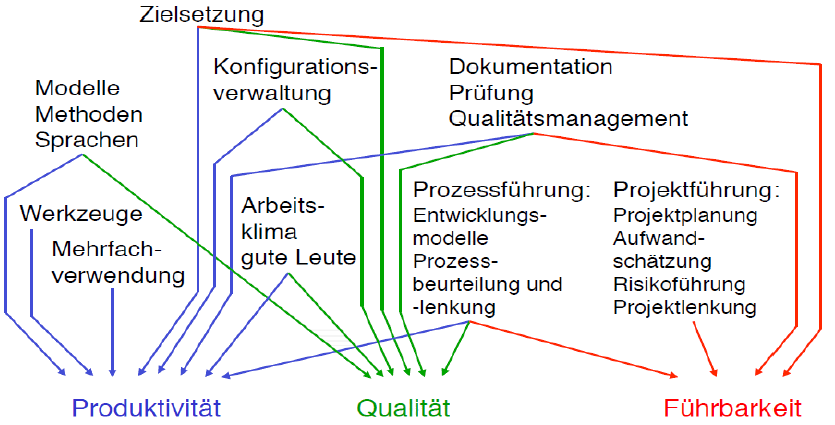
\includegraphics[width=150px]{img/ZieleMittel.png}
        \captionof{figure}{Ziele und Mittel der SE}
        \label{fig:Ziele und Mittel der SE}
    \end{Figure}


\subsection{5 P im Software Engineering}
\begin{itemize}
   \item Projekte
   \subitem klein, gross, sehr gross
   \subitem Forschungsprojekt, Wartungsprojekt
   \subitem Budget, Zeit, Risiko 
   \item Personen
   \subitem Rollen (BA, Architekten, Entwickler, Tester)
   \item Prozesse
   \subitem Vorgehensmodelle (Phasen, Aktivitäten, Vorlagen)
   \subitem Wasserfall, Unified Process, Hermes, Agile
   \item Produkte und Leistungen
   \subitem Artefakte (Zwischenprodukte, Endprodukte)
   \subitem Qualität (Messung, Metriken)
   \item Paradigmen
   \subitem Strukturierte Analyse, Objekt-orientiert, Service-Oriented-Architecture (SOA), Patterns
\end{itemize}

\section{Software Entwicklung als Prozess}
Es gibt einen Produktlebenszyklus, welcher bei der ersten Idee startet und bei der Ausmusterung der Softwarelösung endet.\\
Ein Prozess hilft dabei, dass man schlussendlich zu dem Endprodukt kommt, welcher man entsprechend auch möchte.\\
Ein Softwareprozess ist dann fertig, wenn die Software ausgemustert wurde und \textbf{NICHT} wenn die Software live geht.

\begin{Figure}
   \centering
    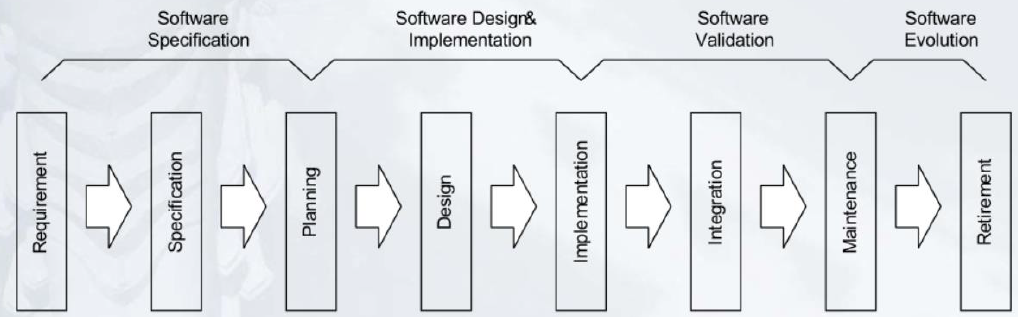
\includegraphics[width=150px]{img/SoftwareLifeCycle.png}
        \captionof{figure}{Übersicht über den Software Lifecycle Prozess}
        \label{fig:Software Lifecycle}
\end{Figure}

\begin{Figure}
   \centering
    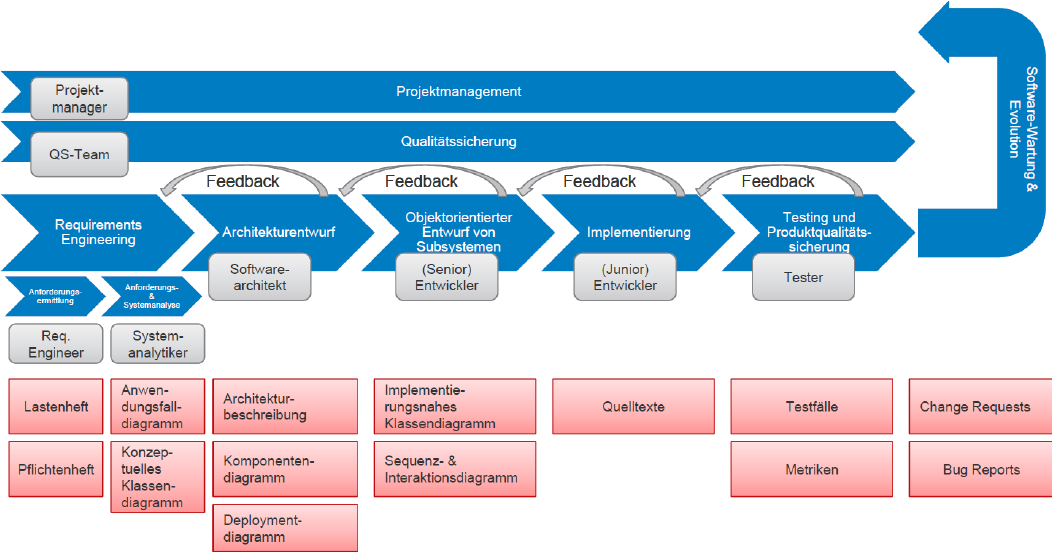
\includegraphics[width=150px]{img/SERoles.png}
        \captionof{figure}{Software Engineering Aktivitäten, Rollen und Artefakten}
        \label{fig:Software Engineering Prozessueberblick}
\end{Figure}

\subsection{Application Lifecycle Management}
Ist in dire Bereichen aufgeteilt:
\begin{itemize}
   \item Governance (Steuerung)
   \item Development (Entwicklung)
   \item Operations (Betrieb)
\end{itemize}

Zusammengehörend ist hierbei auch DevOps (Development - Operations), welches zur Koppelung von Entwicklung und Betrieb führt

\section{Qualitätsaspekte}
für die Produktqualität ist mit ISO 25010 klar definiert. Dabei gibt es interne und externe Qualitäten 

\begin{Figure}
   \centering
    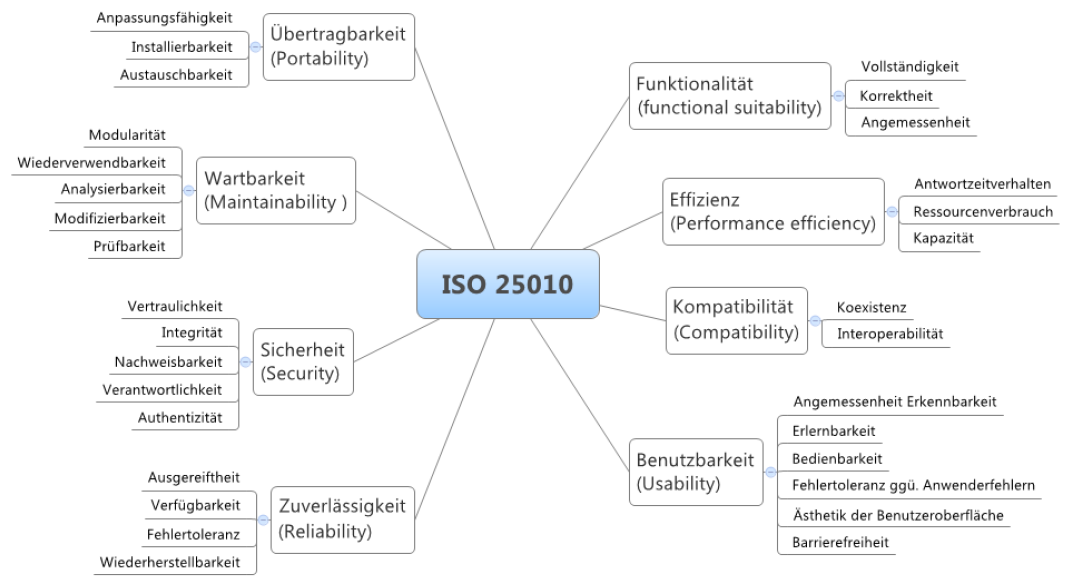
\includegraphics[width=150px]{img/ISO25010.png}
        \captionof{figure}{Qualität gemäss ISO 25010}
        \label{fig:Qualitaet gemaess ISO 25010}
\end{Figure}
$\Rightarrow$ Um die Qualität zu testen, braucht man klare Metriken / Messwerte $\rightarrow$ Hierbei hilft dann beispielsweise das automatische Testen 


\section{SWEBOK}

\chapter{Software Engineering Prozesse}
Ein strukturierter Prozess drängt sich für die Software-Entwicklung auf

\section{Software-Prozessmodelle}
   \subsection{Begrifflichkeiten}
\textbf{Prozess:} Ablauf eines Vorhabens mit der Beschreibung der Schritte (Aktivitäten), der beteiligten Personen (Rollen),
der für diesen Ablauf benötigten Informationen und der dabei entstehenden Informationen (Artefakte)\\

\begin{itemize}
   \item Entwicklung und Wartung von Software sind Prozesse
   \item Ein (Software)
\end{itemize}

   \subsection{Klassifizierung von Software-Entwicklungsprobleme}
   \begin{Figure}
      \centering
       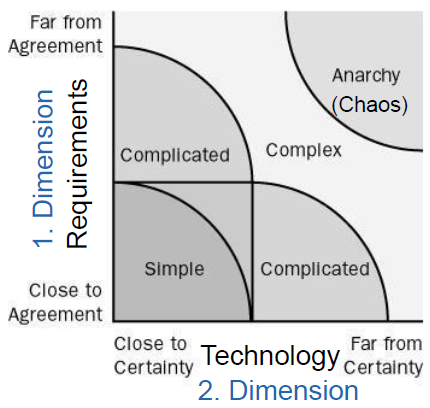
\includegraphics[width=150px]{img/AgilePM.png}
           \captionof{figure}{Einordnung von Probleme}
           \label{fig:Agile Project Management with Scrum}
   \end{Figure}
   \begin{itemize}
      \item heutzutage gibt es keine simple-Projects mehr
      \item häufig sind die Requirements sehr komplex und häufig auch die Technology $\rightarrow$ endet häufig im \textit{complicated} oder \textit{complex} Part
      \item Dazu sollte eigentlich noch eine 3. Dimension gehören $\rightarrow$ Die Menschen (Skills, Intelligence Level, Experience, Attitudes, Prejudices)
   \end{itemize}

\subsection{Aspekte des Softwareentwicklungsprozess}
\begin{itemize}
   \item Ermitteln und Analyse der Anforderungen
   \item Architektur / Entwurf (Design)
   \item Implementierung / Umsetzung (Construction)
   \item Test (Testing)
   \item Inbetriebnahme (Deployment, Configuration, Start of Operation)
   \item Wartung / Betrieb (Maintenance / Operation)
\end{itemize}


\section{Tailoring des Prozesses für ein Projekt}

\chapter{Requirements Engineering}

\section{RE agilen Software-Prozessmodellen}
Aus klassischer Sicht, fixiert man die Requirements und schätzt die Zeit, welche man dazu verwendet.\\
Die neue Methode kehrt dieses Dreieck um, man fixiert die Ressourcen und Zeit und schätzt die Requirements
\begin{Figure}
   \centering
    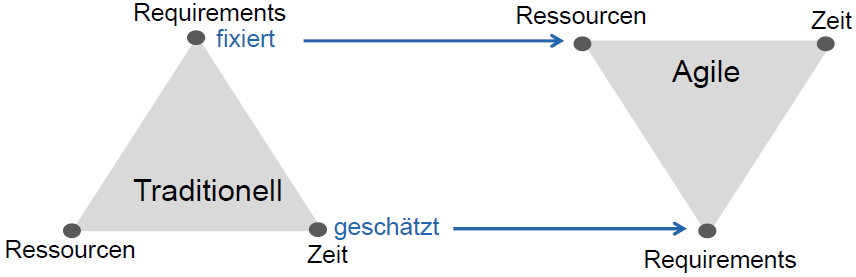
\includegraphics[width=150px]{img/REToday.png}
        \captionof{figure}{Vergleich von RE von früher zu heute}
        \label{fig:Vergleich des Requirements Engineerings von frueher zu heute}
\end{Figure}
Vorteil: Der Kunde weiss noch nicht im Detail, welche Funktionalitäten man erhält, jedoch weiss man wie viel man entsprechend zahlt.

\section{Einführung und Grundlagen}
Warum scheitern Projekte?
\begin{itemize}
   \item Unklare Anforderungen und Ziele
   \item Schlechte Kommunikation
   \item Mangelhaftes Stakeholdermanagement
\end{itemize}
$\rightarrow$ Je später man einen Fehler findet, desto teurer wird dieser Fehler zu reperarien

\subsection{Gründe und Symptome für mangelhaftes RE}
\begin{itemize}
   \item Kommunikationsprobleme
   \item Ergebnisorientierung $\rightarrow$ zu wenig Wert auf Diskussion
   \item Selbstverstständlihckeiten $\rightarrow$ vieles wird angenommen und wird nicht explizit genannt
   \item Projektdruck $\rightarrow$ Auftraggeber erwarten kurzfristige Ergebnisse 
\end{itemize}

\subsection{Risiken bei nicht korrektem Erfassen von Requirements}
\begin{itemize}
   \item Fehlende Anforderungen
   \item ungenaue und falsche interpretierte Anforderungen
   \item Unechte Anforderungen
   \item implizite Anforderungen
   \item widersprüchliche Anforderungen
   \item Schleichende Änderung der Anforderungen
\end{itemize}

\textbf{Anforderung}\\
IEEE-Norm: \textit{Eine Bedingung oder Fähigkeit, die von einem Benutzer (Person oder System) zur Lösung eines Problems oder zur Erreichung eines Ziels benötigt wird}\\

\textbf{Stakeholder}\\
Ein Stakeholder eines Systems ist
\begin{itemize}
   \item eine Person, Personen gruppe oder eine Organisation
   \item die direkt oder indirekt 
   \item Einfluss auf die Anforderungen des betrachteten Systems hat 
\end{itemize}

\textbf{Requirements Engineering}\\
RE ist ein systematischer und disziplinierter Ansatz zur Spezifikation und zum Management von Anforderungen mit folgenden Ziele:
\begin{enumerate}
   \item Die relevanten Anforderungen zu kennne, Konsens unter den Stakeholder über die Anforderungen herstellen, die Anforderungen konform zu vorgegebenen Standards zu dokumentieren und die Anforderungen systematisch zu managen 
   \item Die Wünshce und Bedürfnisse der Stakeholder zu verstehen, zu dokumentieren sowie die Anforderungen zu spezifizieren und zu managen, um das Risiko ....
\end{enumerate}

\subsection{Haupttätigkeiten}
\begin{itemize}
   \item Ermitteln
   \subitem Anforderungen der Stakeholder zu gewinnne, zu detaillieren und zu verfeinern 
   \item dokumentieren
   \subitem Anforderungen adäquat beschreiben
   \item Prüfen und abstimmen
   \subitem Erfüllen der Qualitätskriterien für Anforderungen prüfen
   \item verwalten
   \subitem Anforderungen strukturieren
   \subitem für unterschiedliche Rollen aufbereiten
   \subitem konsistent zu ändern und umzusetzen
\end{itemize}

\subsection{Einflussfaktoren}
Dabei spielt die Domäne und die Umgebung einen wichtige Rolle, diese gelten als Einflussfaktoren.
\begin{itemize}
   \item Anwendungstyp
   \item Anwendungsdomäne
   \item Räumliche Verteilung
\end{itemize}
Des Weiteren ist die Organisation und Prozesse relevant:
\begin{itemize}
   \item Prozesse (Scru, RUP, Hermes etc.)
   \item Best Practices
   \item Normen und Standards (IEEE, ISO, DIN)
\end{itemize}

\subsection{Kommunikation}
Es gibt verschiedene Arten der Kommunikation (schriftlich, mündlich), dabei ist bei dieser Kommunikation wichtig, dass man eine gemeinsame Sprache entwickelt.\\
Dadurch kann man sicherstellen, dass die Fehlerquellen möglichst minimiert werden. Denn der Sender und Empfänger codieren bzw. decodieren jeweils die Nachrichten.

\begin{Figure}
   \centering
    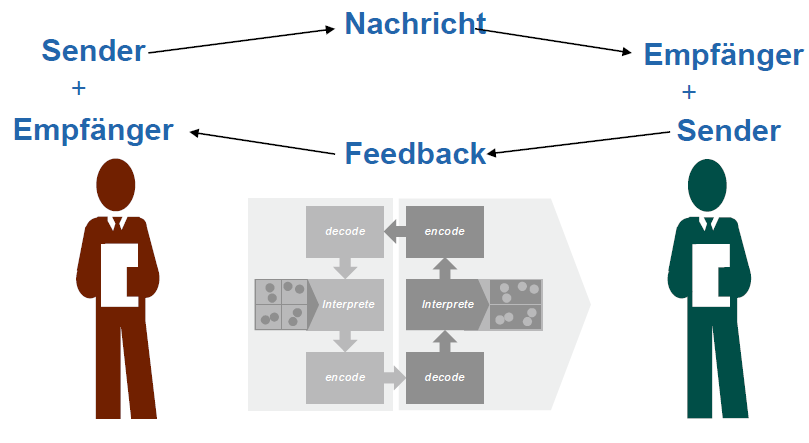
\includegraphics[width=150px]{img/SenderEmpfaenger.png}
        \captionof{figure}{Modell des Sender und Empfaengers}
        \label{fig:Modell des Sender und Empfaengers}
\end{Figure}

Die zwischenmenschliche Kommunikation bewegt sich immer auf zwei Ebenen:
\begin{enumerate}
   \item Inhaltsebene
   \subitem rationaler, sachlicher Austausch von Informationen 
   \item Beziehungsebene
   \subitem Emotionen, bewusst und unbewusste Wahrnehmungen und Gefühle
   \subitem Es sind vielmehr häufig Probleme auf der Beziehungsebene, die eine rationale, sachliche Kommunikation zwischen vers. Personen oder Gruppen erschweren
\end{enumerate}

\subsection{Was sind wichtige Anforderungen an einen Requirements Engineer}
\begin{itemize}
   \item Analytisches Denken
   \item Empathie
   \item Kommunikationsfähigkeit
   \item Konfliktlösungsfähigkeit
   \item Moderationsfähigkeit
   \item Selbstbewusstsein
   \item Überzeugungsfähigkeit
\end{itemize}

   \subsubsection{Requirements Engineer vs. Product Owner}
RE:
\begin{itemize}
   \item Anforderungsermittlung
   \item Anforderungsdokumentation bzw. Wissensvermittlung
   \item Anforderungsvalidierung
   \item Anforderungsmanagement
\end{itemize}

PO:
\begin{itemize}
   \item Sicherstellen, dass das Entwicklungsteam konstanten betriebwirtschaftlichen Wert liefert
   \item Managen aller Stakeholder
   \item Kontinuierliche Versorgung des Entwicklungsteams mit den hochrangigen Einträgen aus dem Backlog
\end{itemize}

$\Rightarrow$ Die Rolle des PO ist breiter gefächert als ein herkömmlicher RE

\subsection{die 3 Arten von Anforderungen}
\begin{itemize}
   \item Funktionale Anforderung
   \item Qualitätsanforderungen $\rightarrow$ Grosser Einfluss auf die Systemarchitektur
   \item Randbedingungen $\rightarrow$ Schränken den Lösungsansatz ein
\end{itemize}
$\rightarrow$ Qualitätsanforderungen und Randbedingungen werden oftmals als \textit{Nicht-funktionale Anforderungen} zusammengefassst.

   \subsection{Qualitätsanforderungen}
Qualitätsanforderungen müssen explizit dokumentiert werden

   \subsection{Wechselwirkung zwischen Was und Wie}
\begin{Figure}
   \centering
    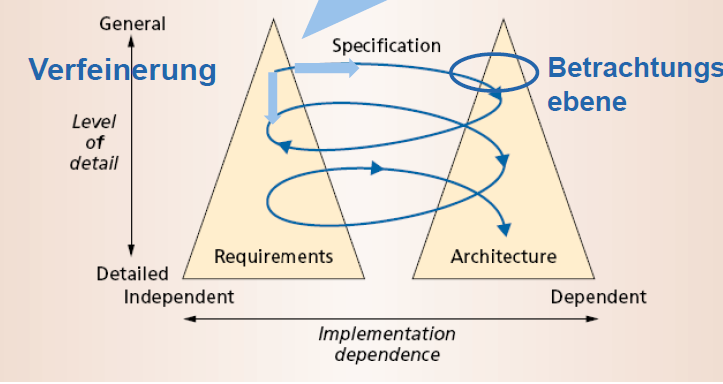
\includegraphics[width=150px]{img/WasWieModell.png}
        \captionof{figure}{Wechselwirkung zwischen Was und Wie}
        \label{fig:Wechselwirkung zwischen Was und Wie}
\end{Figure}

   \subsubsection{Granularität von Anforderungen}

   \begin{Figure}
      \centering
       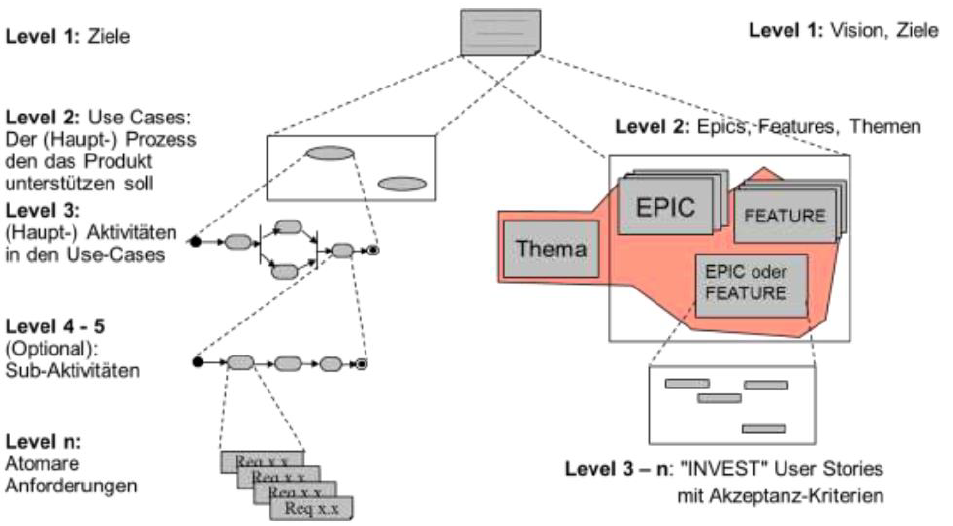
\includegraphics[width=150px]{img/GranularitaetAnforderungen.png}
           \captionof{figure}{Granulariaet von Anforderungen}
           \label{fig:Granulariaet von Anforderungen}
   \end{Figure}

   \begin{Figure}
      \centering
       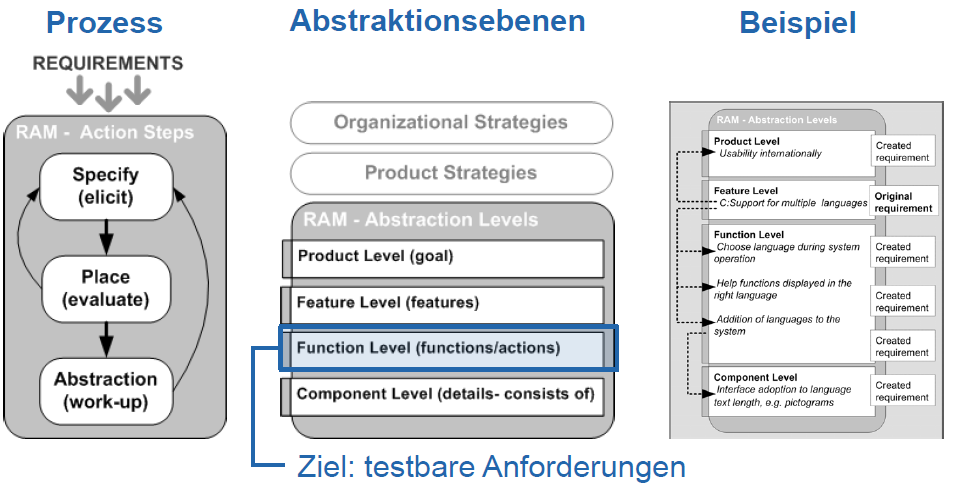
\includegraphics[width=150px]{img/AnforderungsEbene.png}
           \captionof{figure}{Detaillierungsebene}
           \label{fig:Detaillierungsebene}
   \end{Figure}

\subsection{wrap-up}
\begin{itemize}
   \item Gutes RE ist wichtig, da viele Fehler schon in dieser Phase entstehen
   \item Symptome für mangelhaftes RE sind fehlende und unklare Anfoderungen
   \item Vier Haupttätigkeiten (Ermitteln, Dokumentieren, Prüfen, Verwalten)
   \item Sprache ist das wichtigste Mittel der Kommunikation
   \item wichtige Eigenschaften (analytisches Denken, Empathie, Konfliktlösungsfähigkeit, Moderationsfähigkeit, Selbstbewusstsein, Überzeugungsfähigkeit)
   \item drei Arten von Anforderungen (funktionale Anfoderungen, Qualitätsanforderungen, Randbedingungen)
\end{itemize}

\section{System und Systemkontext abgrenzen}
\begin{Figure}
   \centering
    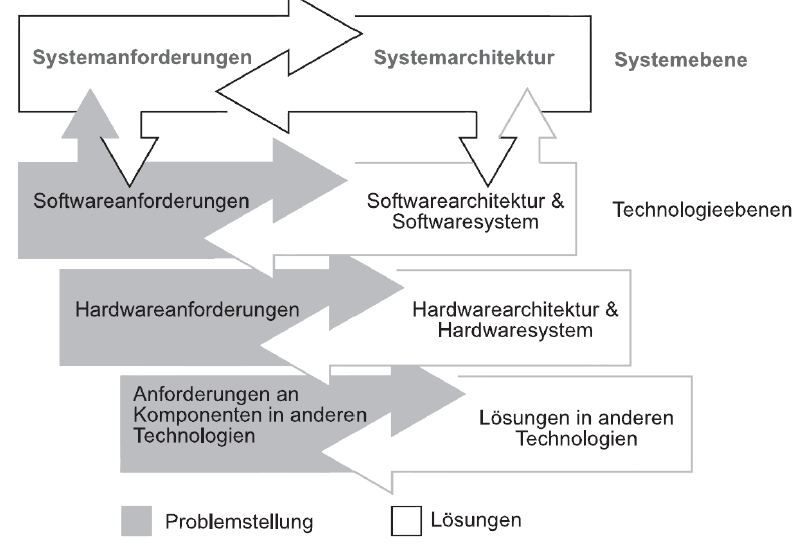
\includegraphics[width=150px]{img/Systembegriffe.png}
        \captionof{figure}{Uebersicht der Systembegriffe}
        \label{fig:Uebersicht der Systembegriffe}
\end{Figure}

\textbf{Systembegriff:}
\begin{itemize}
   \item Unterscheidung von System 
   \item Ein System ist ein dynamisches Ganzes
   \subitem bestmmte eigenschaften und Verhaltensweise
   \subitem besteht aus Teilen die miteinander verknüpft sind
   \subitem das Verhalten des Ganzen beeinflusst wird ... 
   \item Problemstellung und Lösung sollte klar getrennt sein
   \subitem Problemstellung ist meist länger stabil, als die Lösung
   \subitem Zu einer Problemstellung findet man normalerweise mehr als eine mögliche Lösung 
\end{itemize}

$\Rightarrow$ Aus diesen Gründen streben wir die getrennte Formulierung von Problemstellung und Lösung auf jeder Ebene der Entwicklung an
\begin{Figure}
   \centering
    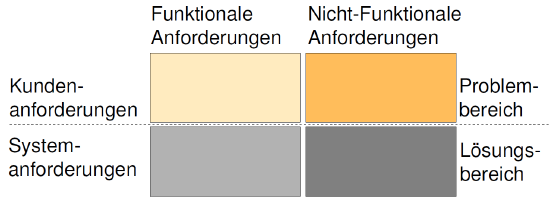
\includegraphics[width=150px]{img/FormulierungProblemstellung.png}
        \captionof{figure}{Formulierung Problemstellung}
        \label{fig:Formulierung Problemstellung}
\end{Figure}

\subsection{Systemgrenze und Umwelt}
Die Systemgrenze speariert das geplante System von seiner Umgebung
\begin{itemize}
   \item gestaltbaren und veränderbarer Teil der Realität von Aspekten in der Umgebung
   \item Es ist zu achten, dass Elemente innerhalb des Systems eine höhrere Verbindungsdichte
\end{itemize}

\subsubsection{Systembetrachtung}
\textbf{1. Wirkung nach aussen:}
\begin{itemize}
   \item Man betrachtet das System als Blackbox
   \item Fokus auf Input und Autbut
\end{itemize}

\textbf{2. Strukturorientiert:}
\begin{itemize}
   \item Strukturorientierte Systembetrachtet
   \item Man bricht das System auf und definiert aus welchen Elementen das System besteht
\end{itemize}

\subsection{Systemkontext}
\textbf{Definition:} \textit{Der Systemkontext ist der Teil der Umgebung eines Systems, der für die Definition und das Verständnis der Anforderungen des betrachteten Systems relevant ist}
\begin{itemize}
   \item Identifikation der materiellen und immateriellen Aspekten, die eine Bezihungs zum System haben 
   \item Der für die Anforderung des System relevante Ausschnit der Realität wird als Systemkontext bezeichnet
\end{itemize}

\subsubsection{Aspekte}
tbd

\subsubsection{Konsequenzen eines fehlerhaften oder unvollständigen Kontextes}
\begin{itemize}
   \item Unvollständige oder fehlerhafte Systemkontexte führen zu fehlerhaften Anforderungen
   \item Entwicklung wird aufgrund von unvollständigen oder fehlerhaften Anforderungen durchgeführt
   \item Diese Fehler bleiben bei der Überprüfung, ob das System die spezifizierten Anforderung abdeckt, unentdeckt. Fehler treten erst später im Betrieb auf.
\end{itemize}

\subsubsection{Systemkontext und Anforderungskontext}
\begin{itemize}
   \item Ursprung der Anforderung eines Systems lieg tim Systemkontext
   \item Eine Anforderung ist in einem spezifischen Kontext definiert
   \item Je vollständiger dieser Kontext einer Anforderung definiert ist, umso geringer ist die Wahrscheinlichkeit der Fehlinterpretation
\end{itemize}

\section{System- und Kontextgrenzen bestimmen}
\begin{itemize}
   \item \textbf{Systemabgrenzung:} Welche Aspekte werden durch das geplante System abgedeckt
   \item \textbf{Kontextabgrenzung:} Grenze des Kontext zur irrelevanten Umgebung
\end{itemize}

\begin{Figure}
   \centering
    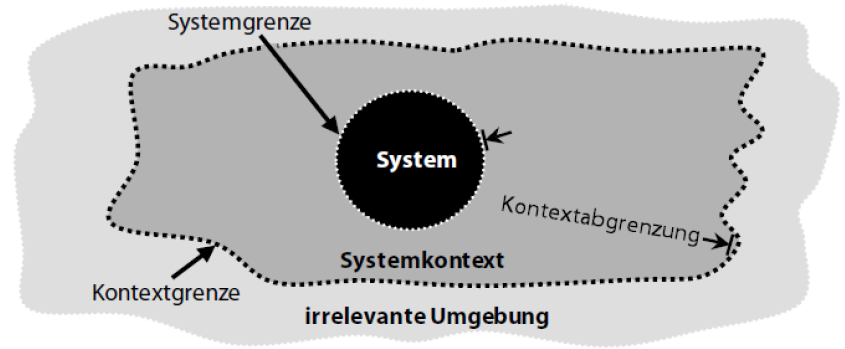
\includegraphics[width=150px]{img/Abgrenzung.png}
        \captionof{figure}{System- und Kontextabgrenzung}
        \label{fig:System- und Kontextabgrenzung}
\end{Figure}

\subsection{Systemgrenze festlegen}
\textbf{Definition Systemgrenze}: \textit{Die Systemgrenze separiert das geplante System von seiner Umgebung.
Sie grenzt den im Rahmen des Entwicklungsprozesses gestaltbaren und
veränderbaren Teil von Aspekten der Umgebung ab, die durch den
Entwicklungsprozess nicht verändert werden können.}
\begin{itemize}
   \item Die Systemgrenze grenzt den Konstruktionsgegenstand zur Umgebung hin ab
   \item Durch die Wahl der Systemgrenze wird festgelegt, welche Aspekte das zu konstruierende System (scope) abdeckt und was ausserhalb des Systems liegt
   \item Sämtliche Aspekte die innerhalb der Systemgrenze liegt, können somit verändert bzw gestaltet werden
\end{itemize}

\subsubsection{Grauzone}
\begin{itemize}
   \item Die Systemgrenze ist oft erst gegen Ende des RE Prozesses präzise festgelegt
   \item Zu Beginn sind bspw. einige oder mehrere Schnittstellen nur Unvollständig bekannt
   \item Die Grauzone kann während dem Prozess laufend verschoben werden
\end{itemize}

\subsubsection{Kontextgrenze bestimmen}
\textbf{Definition:} \textit{Die Kontextgrenze separiert den relevanten Teil der Umgebung eines
geplanten Systems vom irrelevanten Teil, d.h. dem Teil der Umgebung,
der keinen Einfluss auf das geplante System und damit auch keinen
Einfluss auf die Anforderungen dieses Systems hat.
BSc I Modul ASE1 LE 03 - RE Kap. 2 System und Systemkontext abgrenzen}
\begin{itemize}
   \item Die Kontextgrenze differenziert in der Umgebung des geplanten Systems zwischen Kontextaspekte und Aspekte die nicht relevant sind
   \item diese werden idealerweise explizit niedergeschrieben, dass eine impliziten Annahmen getroffen werden können
\end{itemize}

\subsection{Systemkontext dokumentieren}
Diese Dokumentation kann auf unterschiedliche Arten dokumentiert werden
\begin{itemize}
   \item Datenflussdiagrammen
   \item Use Case Diagramme
\end{itemize}
$\rightarrow$ Ist ein sehr einfache Art und Weise mit den Stakeholdern die Grenzen zu definiernen

\begin{Figure}
   \centering
    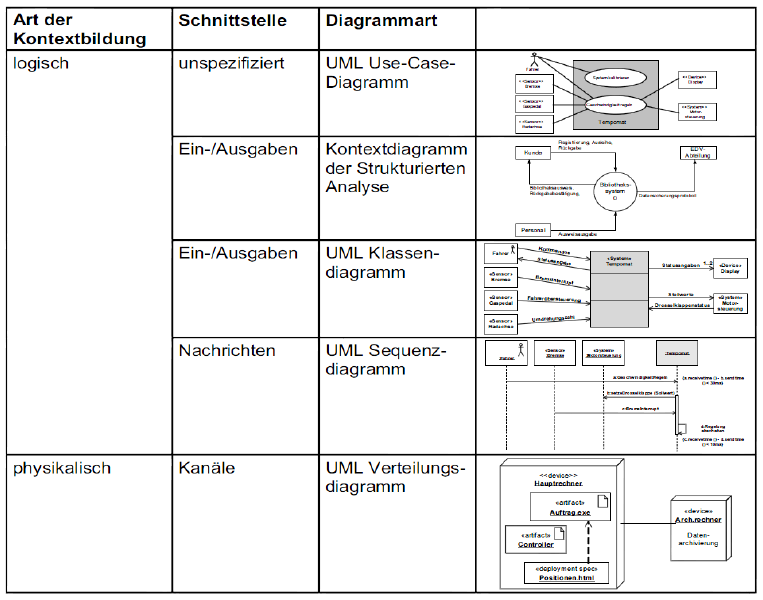
\includegraphics[width=150px]{img/ArtenSystemkontextDoku.png}
        \captionof{figure}{Arten der Dokumentation von Systemkontext}
        \label{fig:Arten der Dokumentation von Systemkontext}
\end{Figure}

\section{Anforderungen ermitteln}

\subsection{Anforderungsquellen}
\begin{itemize}
   \item Stakeholder
   \subitem Person oder Organisation, die Einfluss auf die Anforderungen hat 
   \item Dokumente
   \subitem enthalten wichtige Informationen, aus denen Anforderungen gewonnen werden können 
   \item Altsysteme
   \subitem Systeme im Betrieb oder Konkurrenzsysteme $\rightarrow$ ergeben Basisanforderungen 
\end{itemize}

\subsubsection{Stakeholder}
\begin{itemize}
   \item Identifikation der Stakeholder ist zentrale Aufgabe des RE
   \item sind wichtige Quellen für Anforderungen
   \item RE hat Aufgabe die oft widersprechenden Anforderungen und Ziele der Stakeholder in Einklang zu bringen
\end{itemize}
\begin{Figure}
   \centering
    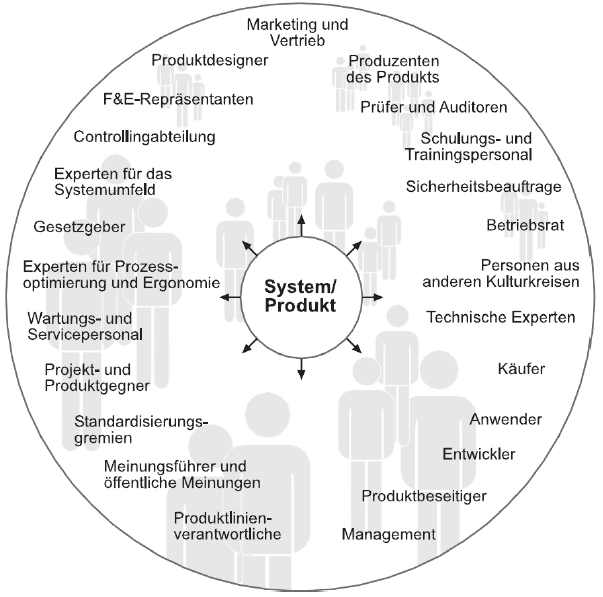
\includegraphics[width=150px]{img/Stakeholder.png}
        \captionof{figure}{Ansicht von versch. Stakeholder}
        \label{fig:Ansicht von versch. Stakeholder}
\end{Figure}

\textbf{Dokumentation}
Die Anforderungsquellen sollte hinsichtlich der Stakeholder dokumentiert werden
\begin{itemize}
   \item normalerweiseFunktion
   \item weitere Personen- und Kontaktdaten
   \item zeitliche und räumliche Verfügbarkeit während Projekt
   \item Relevanz
   \item Wissensgebiet und -umfang
   \item Ziele und Interessen
\end{itemize}

\textbf{Vereinbarungen}
\begin{itemize}
   \item Manchmal lohnt es sich die Aufgaben, Verantwortungsbereiche und Weisungsbefugnisse festzulegen
   \item Dabei geht man auf die Rechte und Pflichte ein 
   \item Dies beugt Mangel an Motivatino bzw. Konflikte vor $\rightarrow$ Stakeholder sollen sich als Projektbeteiligte sehen
\end{itemize}

\subsection{Kano-Model}
Ist für die Anforderungskategorisierung vorgesehen

\begin{itemize}
   \item Basisfaktoren $\rightarrow$ wird als selbstverständlich und absolut notwendig (unbewusste Anforderungen) betrachtet
   \subitem Führt zur massiven Unzufriedenheit
   \subitem Bei Erfüllung gibt es keine positive Stimmung (wird erwartet)
   \subitem Beobachtungstechniken und dokumentenzentrierte Techniken sind guten Ermittlungstechniken
   \item Leistungsfaktoren $\rightarrow$ Sind explizit gewünschte (bewusste) Anforderungen. Der User kann auf einige Leistungsfaktoren verzichten, jedoch nicht auf zu viele
   \subitem Steigert Zufriedenheit
   \subitem gut durch Befragungstechniken zu ermitteln
   \item Begeisterungsfaktoren $\rightarrow$ wird erst durch die Benutzung ersichtlich und begeistert die Nutzer zusätzlich
   \subitem unbewusste Anforderungen - werden nicht erwartet
   \subitem durch Kreativitätstechniken gut zu ermitteln 
\end{itemize}

\begin{Figure}
   \centering
    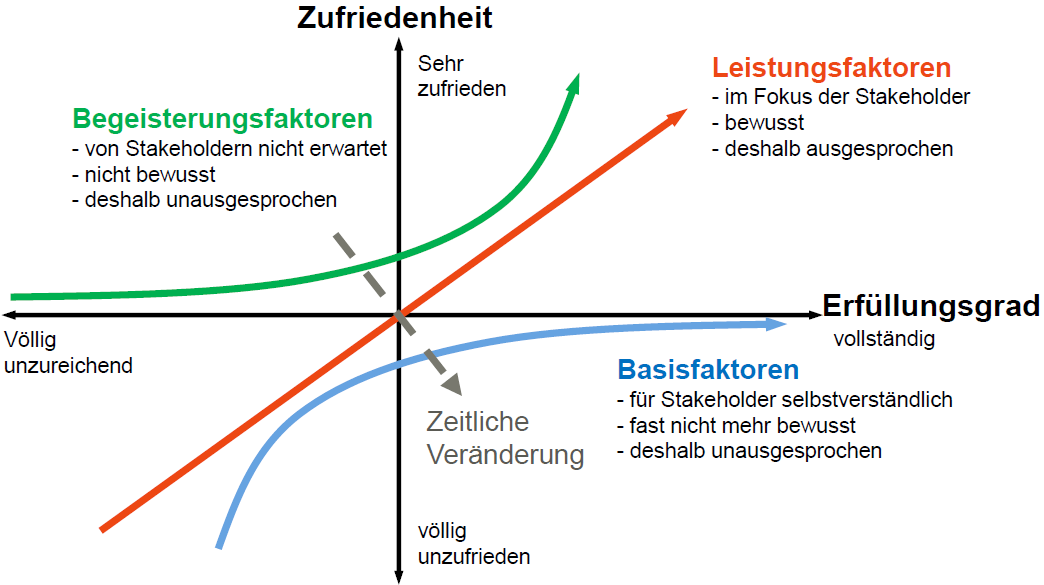
\includegraphics[width=150px]{img/KanoModell.png}
        \captionof{figure}{Ansicht der verschiedenen Anforderungskategorisierung}
        \label{fig:Ansicht der verschiedenen Anforderungskategorisierung}
\end{Figure}
$\Rightarrow$ Mit der Zeit wird ein Begeisterungsfaktor zu einem Leistungsfaktor und anschliessend zu einem Basisfaktor

\subsection{Ermittlungstechniken}
Ermittlungstechniken erfüllen den Zweck, die bewussten, unbewussten und unterbewussten Anforderungen der Stakeholder herauszufinden.
\begin{itemize}
   \item Ergebung ist zeit- und arbeitsintensiv
   \item ein geeigneter Satz an Techniken muss pro Projekt aufeinander abgestimmt werden
   \item Jede Erhebung benötigt mehrere Runden
\end{itemize}

\begin{itemize}
   \item Befragungstechniken
   \subitem Interview
   \subitem Fragebogen 
   \item Kreativitätstechniken
   \subitem Brainstroming
   \subitem Brainstroming paradox
   \item dokumentenzentrierte Techniken
   \item Beobachtungstechniken
   \item unterstützende Techniken
\end{itemize}
$\Rightarrow$ Die Technikwahl ist massgebend für den Erfolg

\begin{Figure}
   \centering
    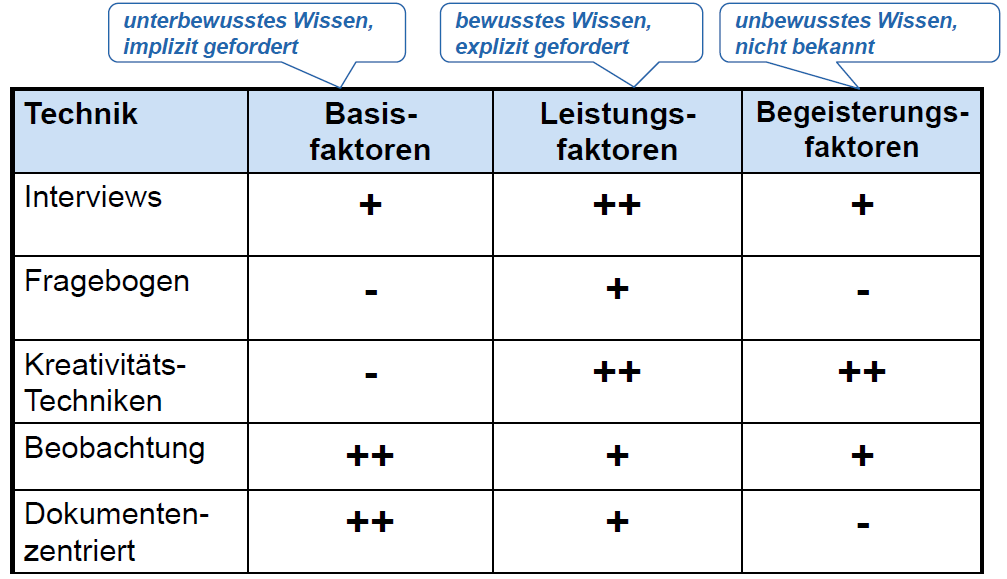
\includegraphics[width=150px]{img/ErmittlungstechnikenKanoModell.png}
        \captionof{figure}{Zusammenhang Ermittlungstechniken mit dem Kano-Modell}
        \label{fig:Zusammenhang Ermittlungstechniken mit dem Kano-Modell}
\end{Figure}

\begin{itemize}
   \item Unterscheidung je nach Anforderungen
   \item Termin- und Budgetvorgaben
   \item Verfügbarkeit der Stakeholder
   \item Erfahrung des RE
   \item Chancen und Risiken des REs
\end{itemize}

\textbf{Risikofaktoren}
\begin{itemize}
   \item Menschliche Einflüsse
   \subitem gute Kommunikation, Anforderungsart, Detaillierungsebene, Erfahrung
   \subitem kognitive Fähigkiet der Stakeholder
   \item Organisatorische Einflüsse
   \subitem Festpreis oder Werktvertrag
   \subitem ...
\end{itemize}

\subsubsection{Befragungstechniken}
\begin{itemize}
   \item Aussage des Stakeholders über die Anforderungen an das System aus seiner Perspektive
   \item Stakeholder muss Wissen explizit ausdrücken
   \item tendenziell durch den RE durchgeführt
\end{itemize}

\textbf{Interview}
\begin{itemize}
   \item mehrere vorgegebene Fragen werden gestellt und protokolliert
   \item Fragen werden im Gespräch geklärt
   \item durch geschickte Fragen können unbewusste Anforderungen ermitteln
\end{itemize}
\textit{Vorteile}
\begin{itemize}
   \item sehr direkt und gezielt auf den Sachverhalt eingehen
   \item individuell auf Gesprächspartner anpassbar
   \item Wenige Missverständnisse
\end{itemize}
\textit{Nachteile}
\begin{itemize}
   \item Aufwändige Vorbereitung
   \item Qualität vom Interviewer abhängig
   \item Auswertung ist arbeitsintensiv
\end{itemize}

\textbf{Fragebogen}
\begin{itemize}
   \item offene und oder geschlossene Fragen
   \item gut online möglich
   \item in kurzer Zeit viele Personen befragen
\end{itemize}
\textit{Vorteile}
\begin{itemize}
   \item einfache und schnelle Auswertung
   \item Anonymität möglich
   \item Schriftliche Aussagen können nur schwer dementiert werden
   \item einen Schlag viele Stakeholder 
\end{itemize}
\textit{Nachteile}
\begin{itemize}
   \item nur abgefragt, was der RE bereits kennt oder vermutet
   \item Angst vor schriftlicher Befragung
   \item Einfluss von Drittpersonen möglich
   \item Mangelhaftes Ausfüllen hat mühsame Rückfragen zur Folge
   \item persönlicher Kontakt fehlt
   \item Motivation der Befragten kann geringer sein als bei einem persönlichen Gespräch
\end{itemize}

\subsubsection{Kreativitätstechniken}
\begin{itemize}
   \item Entwicklung von innovativen Anforderungen (Visionen)
   \item nicht für die Ermittlung von detaillierten Anforderungen
\end{itemize}

\textbf{Brainstorming}
\begin{itemize}
   \item 5 - 10 Personen in vorgegebener Zeit Ideen gesammelt
   \item Erst im Anschluss werden diese geprüft und analysiert
\end{itemize}
\textit{Vorteil}
\begin{itemize}
   \item finden von innovativen Ideen und ausgefallenen Lösungen
   \item kann gut in Sackgass-Situationen verwendet werden
   \item Einfache Durchführung
   \item geringe Kosten
   \item Ausnutzung von Synergieeffektive infolge Gruppenbildung
\end{itemize}
\textit{Nachteil}
\begin{itemize}
   \item Stark abhängig der Teilnehmer
   \item Oftmals sehr viel unbrauchbar
   \item Gefahr in Abschweifung
   \item Aufwändige Selektion der Ideen
   \item Gefahr von gruppendynamische Konflikte
\end{itemize}

\textbf{Brainstorming Paradox}
\begin{itemize}
   \item genau gleich wie Brainstorming
   \item Ergebnisse werden gesammelt, welche nicht erreicht werden sollen
\end{itemize}

\text{Perspektivenwechsel}
\begin{itemize}
   \item Arbeitet mit Perspektivenwechsel
   \item bspw. Sechs-hut-Denken (jeder Hut nimmt andere Perspektive ein (neue Idee, Zweifel etc.))
   \item ganzheitliche Betrachtung / animiert neue Sichtweisen einzunehmen
   \item nicht geeignet für Detailarbeiten und Präzison / Akzeptanz der Technik
\end{itemize}

\subsubsection{Dokumentenzentrierte Techniken}
\begin{itemize}
   \item verwenden Lösungen und Ideen von bestehenden Systemen weiter
   \item ...
\end{itemize}

\textbf{Systemarchäologie}
\begin{itemize}
   \item Untersuchender Funktionalitäten eines bestehenden Systems
\end{itemize}


\textbf{Perspektivenbasiertes Lesen und Wiederverwendung}
\begin{itemize}
   \item Perspektivenbasiertes Lesen
   \item Wiederverwendung
\end{itemize}

\subsubsection{Beobachtungstechniken}
\begin{itemize}
   \item RE beobachtet Abläufe und hinterfragt diese
   \item RE hat die Chance ineffiziente Prozesse zu erkennen
\end{itemize}

\textbf{Feldbeobachtung}
\begin{itemize}
   \item RE ist vor Ort 
   \item Dokumentiert unmittelbar vor Ort
   \item Evtl. Audio oder Videoaufzeichnung
\end{itemize}

\textbf{Apprenticing}
\begin{itemize}
   \item RE geht in die Lehre
   \item Arbeitet aktiv mit
   \item UNklare Handlungen werden sofort hinterfragt
   \item Machtverhältnis Stakeholder und RE ist umgedreht
\end{itemize}

\subsubsection{Unterstützende Techniken}
\begin{itemize}
   \item Mindmapping
   \item Workshops
   \item Use Cases Modellierung
   \item User stories
   \item Prototypen
\end{itemize}

\section{Anforderungen dokumentieren}

Einflussfaktoren für das Dokumentieren
\begin{itemize}
   \item Kritikalität
   \item Risiko
   \item Wichtigkeit der Kunden
   \item Rechtliche Verbindlichkeit
   \item Grad der Standardisierung
   \item Erfahrung
\end{itemize}

\subsection{vier Arten von Dokumentation}
\begin{itemize}
   \item Dokumentation für gesetzliche Zwecke
   \subitem Prinzip: muss aus den Gesetzen und Standards abgeleitet werden 
   \subitem ist untrennbarer Bestandteil des Produkts 
   \item Dokumentation zum Zwecke der Bewahrung
   \subitem Prinzip: Das Team entscheidet, was zum Zwecke der Bewahrung dokumentiert wird 
   \item Dokumentation für Kommunikationszwecke
   \subitem Prinzip: zusätzliches Kommunikationsmittel
   \subitem Verlief die Kommunikation erfolgreich, sollte das Dokument archiviert werden
   \item Dokumentation zur Zwecke von Überlegungen
   \subitem Prinzip: nachdenkende Person entscheidet über die Dokumentform
   \subitem muss ihre Wahl nicht rechtfertigen
   \subitem Dokument kann verworfen werden  
\end{itemize}

$\Rightarrow$ Ist kein Selbstzweck, sondern soll die Kommunikation zwischen Stakeholdern erleichertn, vor allem zwischen dem Anfordernden und dem Entwicklungsteam

\begin{Figure}
   \centering
    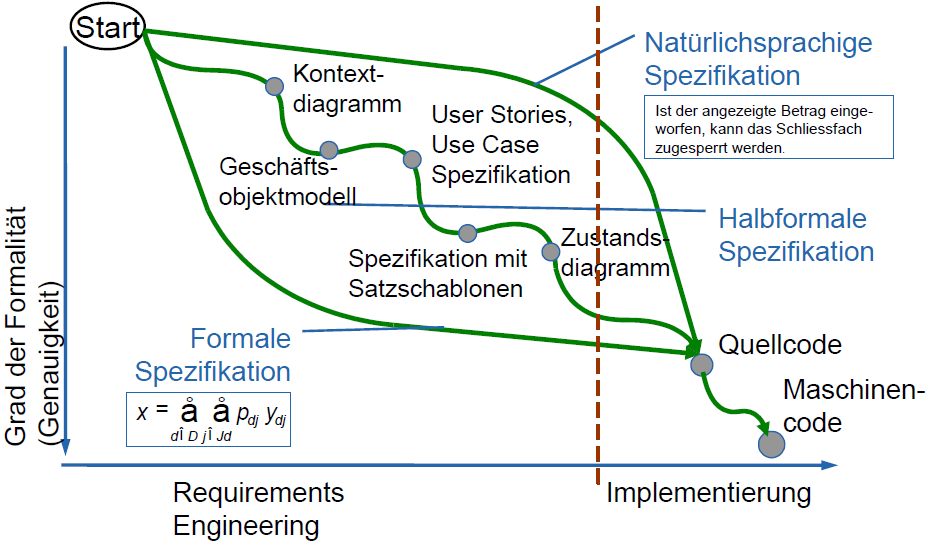
\includegraphics[width=150px]{img/Dokumentationsformen.png}
        \captionof{figure}{Varianten der Dokumentationsformen}
        \label{fig:Varianten der Dokumentationsformen}
\end{Figure}

\subsection{Dokumentengestaltung}
tbd

\subsection{Arten der Dokumentation}
tbd

\subsection{Dokumentenstrukturen}
Standard oder individuelle Dokumentenstruktur\\
Vorteil von Standards:
\begin{itemize}
   \item Einarbeitungszeit kleiner
   \item Schnellere Erfassung von ausgewählter Inhaltsebene
   \item ...
\end{itemize}

Was gibt es für Standards?
\begin{itemize}
   \item RUP - Rational Unified Process (IBM)
   \subitem Enthält untersch. Artefakten 
   \item Standard ISO/IEC/IEEE 29148:2011
   \item V-Modell
   \subitem Lastenheft
   \subitem Pflichtenheft 
\end{itemize}

\begin{Figure}
   \centering
    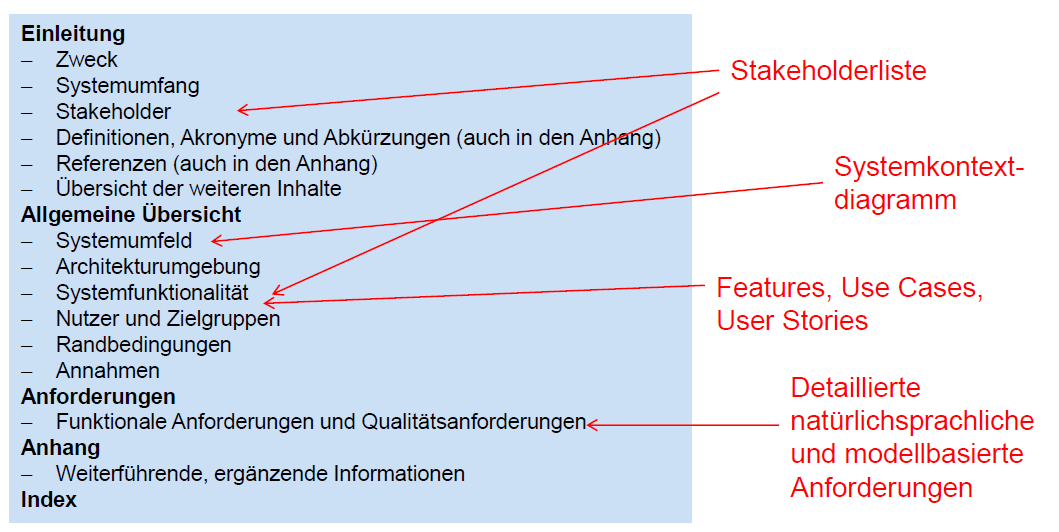
\includegraphics[width=150px]{img/Standardinhalte.png}
        \captionof{figure}{Angepasste Standardinhalte SRS}
        \label{fig:Angepasste Standardinhalte SRS}
\end{Figure}

\subsection{Verwendung von Anforderungsdokumenten}
\begin{itemize}
   \item Planung
   \item Architekturentwurf
   \item Implementierung
   \item Test
   \item Änderungsmanagement
   \item Systemnutzung und Systemwartung
   \item Vertragsmanagement
\end{itemize}

\subsection{Qualitätskriterien für das Anforderungsdokument}
\begin{itemize}
   \item Eindeutigkeit und Konsistenz
   \item Klare Struktur
   \item Modifizierbarkeit und Erweiterbarkeit
   \item Vollständig
   \item Verfolgbarkeit
\end{itemize}

\section{Anforderungen natürlich sprachlich dokumentieren}

\subsection{Sprachliche Effekte}
\begin{itemize}
   \item Realität $\rightarrow$ Tiefenstruktur (Interpretation)
   \item Oberflächenstruktur $\rightarrow$ Tiefenstruktur (Nachfragen)
   \item Durch die sprachlichen Effekte können gleiche Dinge unterschiedliche Interpretation erfolgen
   \item die natürliche Sprache ist mehrdeutig und interpretierbar
   \item bei den Vorgängen Wahrnehmung und Darstellung treten so genannte Transformationsprozesse auf
\end{itemize}

Es gibt funf für das RE relevantesten Transformationsprozesse:
\begin{Figure}
   \centering
    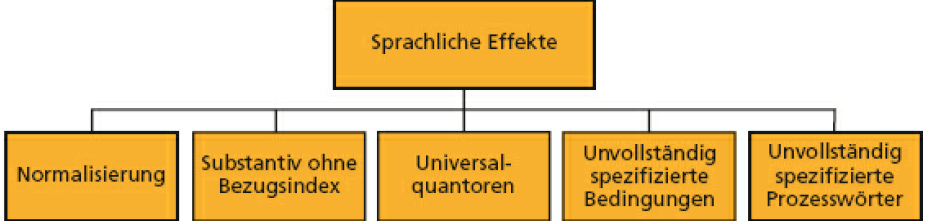
\includegraphics[width=150px]{img/5Transformationsprozesse.png}
        \captionof{figure}{die wichtigsten Transformationsprozesse}
        \label{fig:die wichtigsten Transformationsprozesse}
\end{Figure}

\subsubsection{Normalisierung}
\begin{itemize}
   \item Ähnliche Begriffe in einem Verb zusammenfassen
   \item Durch diese Umwandlung gehen wichtige Informationen verloren
   \item Bei der sprachlichen Analyse werden alle Normalisierungen identifiziert
   \item Schwierigkeit ist, dass bei der Normalisierung jeweils komplexe Prozesse darunterstecken können
   \subitem bspw. Rückgabe $\rightarrow$ Rückgabe muss genauer analysiert werden 
\end{itemize}

\subsubsection{Substantive ohne Bezugsindex}
\begin{itemize}
   \item Substantive bergen ähnliche Prozesswörter die Gefahr der unvollständigen Spezifizierung $\rightarrow$ ohne ausreichende Bezugsindizes
   \subitem bspw. der Anwender, der Daten, das System
   \subitem besser: der angemeldete Anwender 
\end{itemize}

\subsubsection{Universalquantoren}
\begin{itemize}
   \item Universalquantoren sind Angaben über die Häufigkeit
   \item Hinterfragen ob das für alle Objekte gilt
   \subitem bspw: nie, immer, alle, irgendeiner 
\end{itemize}

\subsubsection{unvollständig spezifzierte Bedingungen}
\begin{itemize}
   \item Unvollständige spezifzierte Bedingungen
   \item Eintritt der Bedingung wird beschrieben (if-Fall), aber nicht der Else-Fall
\end{itemize}

\subsubsection{Unvollständig spezifizierte Prozesswörter}
\begin{itemize}
   \item Prozesswörter brauchen mehr als ein Substantiv, um vollständig spezifziert zu sein
   \subitem bspw. übertragen: was? von wo? wohin?
\end{itemize}

\subsection{Konstruktion von Anforderungen mittels Satzschablone}
\begin{itemize}
   \item Ein einfach erlern- und einsetzbarer Ansatz zur Reduzierung sprachlicher Effekte während der Formulierung von Anforderung ist die Satzschablone
   \item Die Satzschablone unterstützt den Autor einer Anforderung effektiv dabei, qualitativ
   \item ...vervollständigen...
\end{itemize}

\textbf{Schritt 1}\\
Das Festlegen der Verbindlichkeit durch die Verben, 'muss', 'sollte', 'wird' kann im Text der Anforderung erfolgen. Ändern sich die Verbindlichkeiten, dann ändern sich auch die Anforderungen

\begin{Figure}
   \centering
    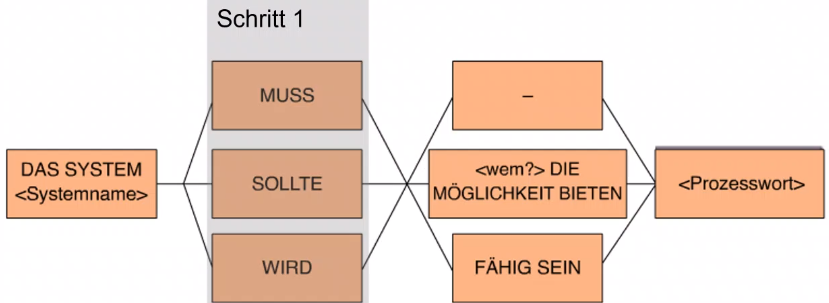
\includegraphics[width=150px]{img/SatzSchablone1.png}
        \captionof{figure}{Schritt eins der Satzschablone}
        \label{fig:Schritt eins der Satzschablone}
\end{Figure}

\textbf{Schritt 2}\\
Geforderte Funktionalität, drucken, speicher, übertragen ist ein Prozess und wird durch Verben beschrieben $\rightarrow$ Gefordertes Systemverhalten wird in Schritt 2 beschrieben
\begin{Figure}
   \centering
    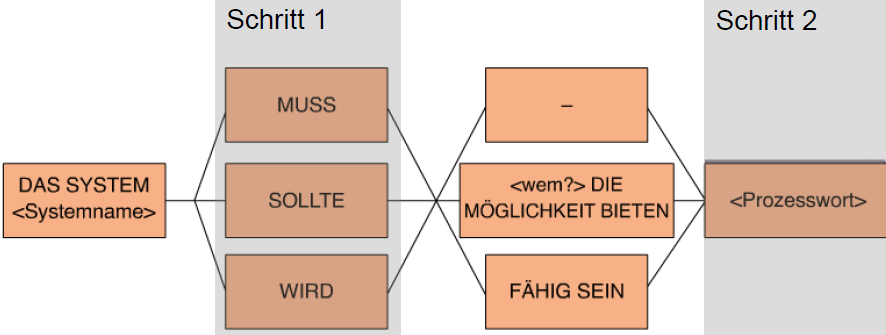
\includegraphics[width=150px]{img/SatzSchablone2.png}
        \captionof{figure}{Schritt zwei der Satzschablone}
        \label{fig:Schritt zwei der Satzschablone}
\end{Figure}

\textbf{Schritt 3}
\begin{itemize}
   \item Selbstständige Systemaktivität
   \subitem Das System führt den Prozess selbstständig durch 
   \item Benutzerinteraktion
   \subitem Das System stellt dem Nutzer die Prozessfunktionalität zur Verfügung 
   \item Schnittstellenanforderungen
   \subitem Das System führt einen Prozess in Abhängigkeit von einem Dritte (bspw. Fremdsystem) aus, ist an sich passiv und wartet auf ein externes Ereignis 
\end{itemize}
\begin{Figure}
   \centering
    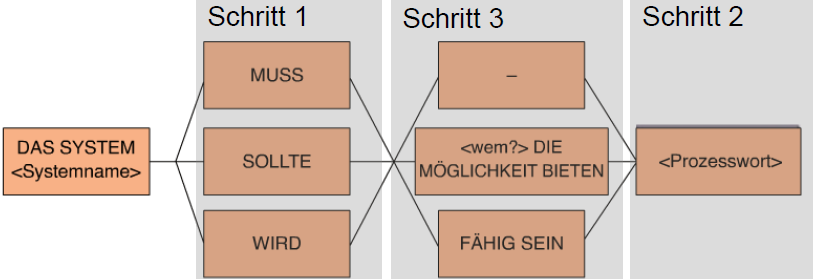
\includegraphics[width=150px]{img/SatzSchablone3.png}
        \captionof{figure}{Schritt drei der Satzschablone}
        \label{fig:Schritt drei der Satzschablone}
\end{Figure}

\textbf{Schritt 4}\\
Manche Prozesswörter benötigen zur Ergänzung ein oder mehrere Objekte $\rightarrow$ das Prozesswort \textit{drucken} wird um was oder wo ergänzt\\

\textbf{Schritt 5}\\
Für Anforderungen ist es typisch, dass die geforderte Funktionalität nicht fortwährend, sondern nur unter bestimmten zeitlichen oder logischen Bedingungen ausgeführt oder zur Verfügung gestellt wird
\begin{itemize}
   \item zeitliche Bedingung (sobald, nachdem)
   \item Logische Bedingung (Falls)
   \item Wenn sollte vermieden werden, weil es zeitlich oder logisch eingesetzt werden kann
\end{itemize}

\begin{Figure}
   \centering
    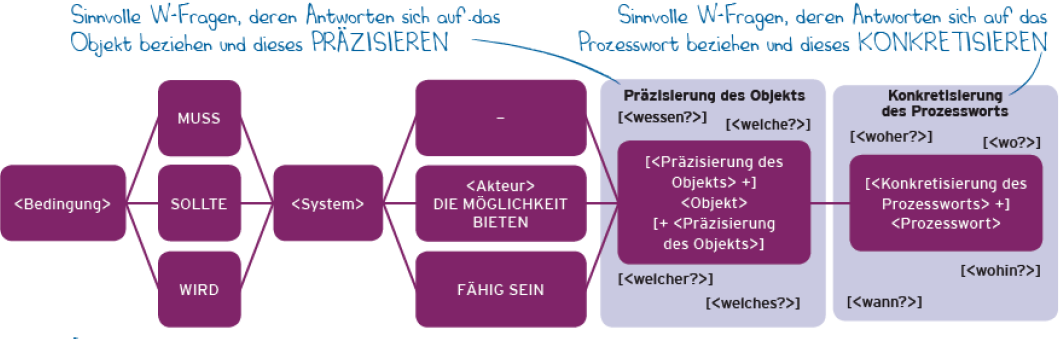
\includegraphics[width=150px]{img/SatzSchablone.png}
        \captionof{figure}{vollstaendige Satzschablone}
        \label{fig:vollstaendige Satzschablone}
\end{Figure}

\section{Anforderungen modellbasiert dokumentieren}

\subsection{Der Modellbegriff}
Ein Modell ist ein abstrahierendes Abbild einer existierenden Realität oder Vorbild für eine zu schaffende Realität
\begin{itemize}
   \item Modelle können nicht falsch oder richtig sein, sondern vielmehr kann passend bzw. nicht-passend für ein System sein
   \item ...
\end{itemize}

\begin{Figure}
   \centering
    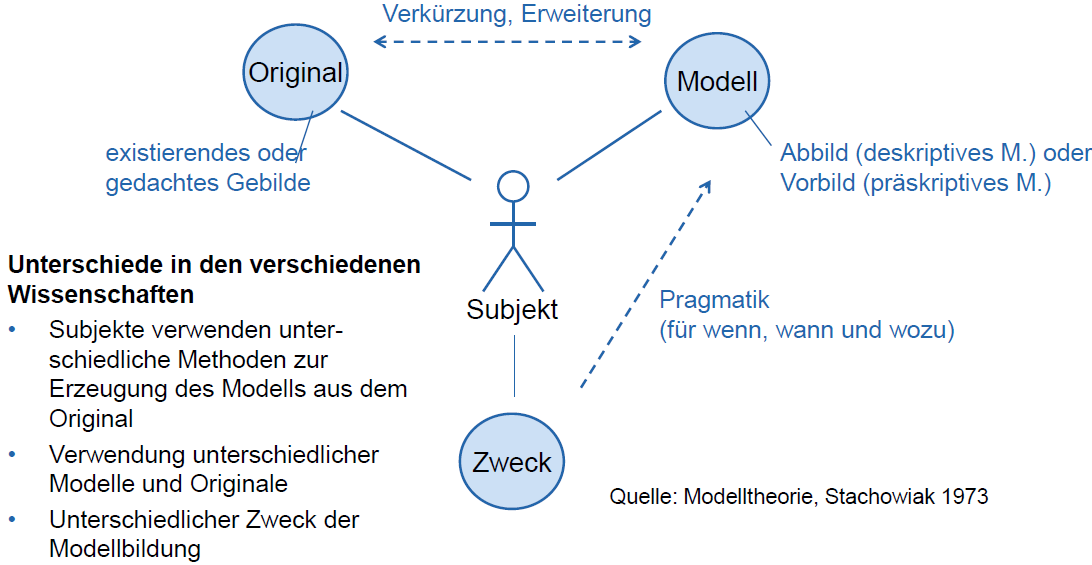
\includegraphics[width=150px]{img/Modelleigenschaften.png}
        \captionof{figure}{Eigenschaften von Modellen}
        \label{fig:Eigenschaften von Modellen}
\end{Figure}

\begin{Figure}
   \centering
    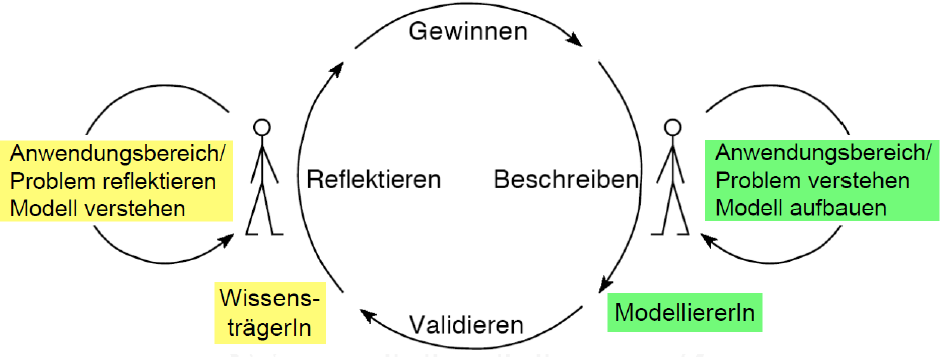
\includegraphics[width=150px]{img/Modellschema.png}
        \captionof{figure}{Prinzipschema von Modellen}
        \label{fig:Prinzipschema von Modellen}
\end{Figure}
\begin{itemize}
   \item Modellbildung ist ein iterativer Prozess
   \item Bedeutet auch immer Refelktieren über das Original
   \item Ist auch ein Verstehens- und Konsesbildungsprozess
\end{itemize}

\textbf{Konzeptuelle Modellierungssprachen}
\begin{itemize}
   \item Konzeptuelle Modelle, die Anforderungen eines Systems dokumentieren, werden als Anforderungsmodelle bezeichnet
   \subitem wird oftmals UML eingesetzt
   \subitem UML besteht aus einer Menge von zum Teil komplementären Modellierungssprachen, die speziell im RE eingesetzt werden um die Anforderungen eines Systems aus verschiedenen Perspektiven zu modellieren
   \subitem Unterschied konzeptuelle Modelle in der Systementwicklung der Verwendung von konzeptuellen Modellen in der Anforderungsdokumentation
   \subsubitem Systementwicklung: es wreden Lösungsaspekte dokumentiert
   \subsubitem RE: es werden Anfordernden aus verschiedenen Perspektiven modelliert
   \item Zur Modellierung Konzeptueller Modelle werden Konzeptuelle Modellierungssprachen eingesetzt, die über deren Syntax (Modellierungselemente und deren gültige Kombination) und Semantik (Bedeutung der Modellierungselemente) definiert werden
   \item Konzeptuelle Modelle können hinsichtlich ihres Formalisierungsgrades in informale, semiformale und formale Modellierungssprache eingeteilt werden
   \item Der Formalisierungsgrad ist abhängig vom Umfang, in dem Syntax und Semantik der Sprache formal definiert sind
\end{itemize}

\textbf{Anforderungsmodelle}
\begin{itemize}
   \item Konzeptuelle Modelle, die Anforderungen eines Systems dokumentieren, werden als Anforderungsmodelle bez
\end{itemize}

\subsection{Zielmodelle}
\begin{itemize}
   \item Ziele $\rightarrow$ Und-Oder-Graphen
   \item Szenarien
   \subitem Personas und Szenarien
   \subitem Storyboards
   \subitem Use Case Diagramme
   \item Funktionsperspektive
   \subitem UML-Aktivitätsdiagramme
   \subitem UML-Sequenzdiagramme
   \subitem Datenflussdiagramme 
   \item Strukturperspektive
   \subitem UML-Klassendiagramme
   \subitem Entity-Relationship-Diagramme 
   \item Verhaltensperspektive
   \subitem UML-Zustandsdiagramme
   \subitem Statecharts
\end{itemize}

\subsection{Use Cases}
Use Cases sind noch nicht alle Anforderungen, sondern werden durch weitere Anforderungen mit UI-Sketches bzw. Prosa definiert
\begin{Figure}
   \centering
    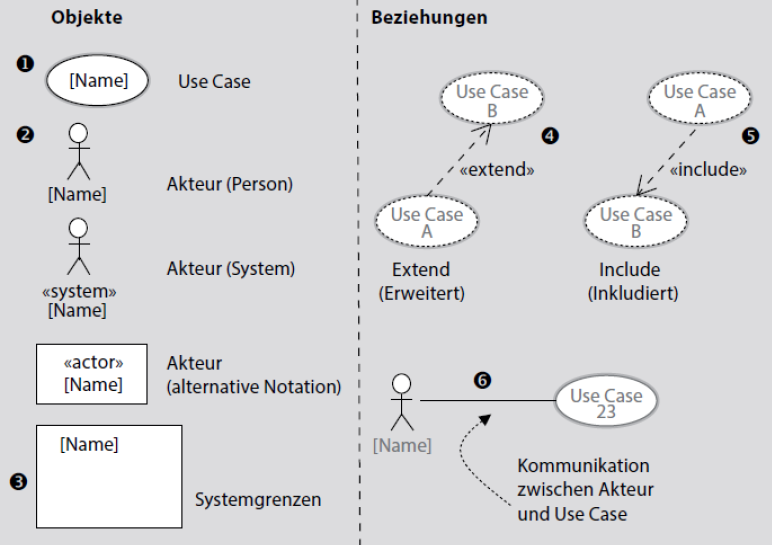
\includegraphics[width=150px]{img/UseCaseElemente.png}
        \captionof{figure}{Modellelemente Use Case}
        \label{fig:Modellelemente Use Case}
\end{Figure}

\textbf{Use Case Spezifikation}
\begin{itemize}
   \item ergänzen die überblicksartigen Use-Case-Diagramme durch eine genaue Spezifikation der wesentlichen Eigenschaften einzelner Use Cases
   \item Hierzu wird i nder Regel für jeden relevanten Use Case spearat eine vorgebene Schablone ausgefüllt
\end{itemize}

\subsection{Drei Prespektiven auf die Anforderungen}

\subsubsection{Anforderungesmodellierung in der Strukturperspektive}
Mit Entity-Relationship-Diagramm (ERD) $\rightarrow$ in der Regel wird jedoch die UML Notation verwendet\\

Häufiger wird mit UML-Klassendiagramme gearbeitet
\begin{Figure}
   \centering
    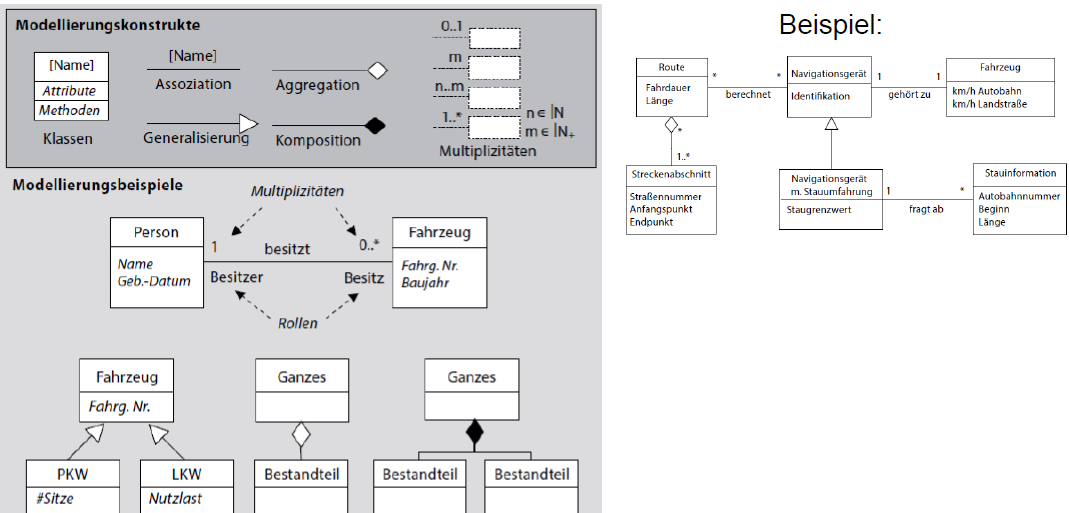
\includegraphics[width=150px]{img/UMLKlassendiagramm.png}
        \captionof{figure}{Elemente des UML Klassendiagramm}
        \label{fig:Elemente des UML Klassendiagramm}
\end{Figure}


\subsubsection{Anforderungesmodellierung in der Funktionsperspektive}
Datenflussdiagramme werden fast nicht mehr verwendet, da veraltet $\rightarrow$ wurde durch UML-Aktivitätsdiagramme abgelöst\\

Das UML-Aktivitätsdiagram:
\begin{Figure}
   \centering
    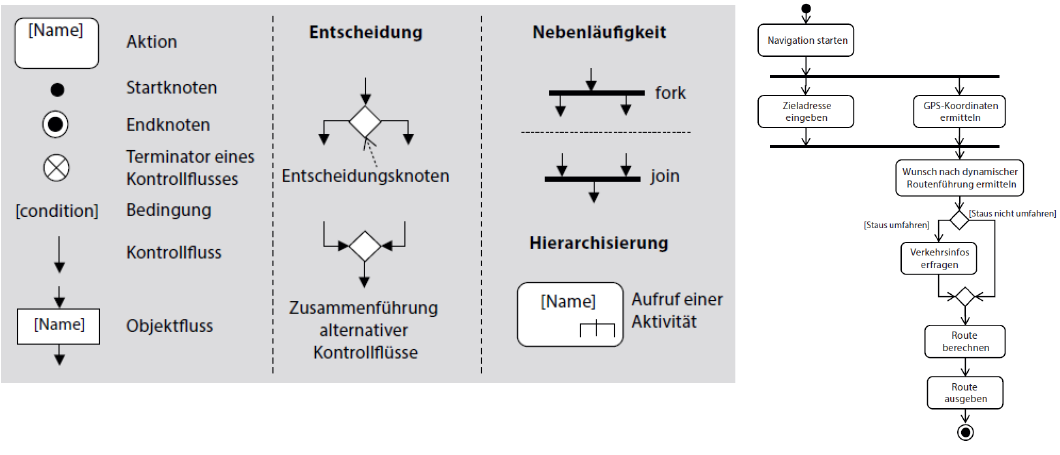
\includegraphics[width=150px]{img/UMLAktivitatsdiagramm.png}
        \captionof{figure}{Elemente des UML Aktivitätsdiagram}
        \label{fig:Elemente des UML Aktivitaetsdiagram}
\end{Figure}
$\Rightarrow$ sehr gut geeignet für das Modellieren von Parallel-Abläufen


\subsubsection{Anforderungesmodellierung in der Verhaltensperspektive}

Statechart ist ebenfalls veraltet $\rightarrow$ wird durch UML-Zustandsdiagramme abgelöst\\

UML-Zustandsdiagramme:
\begin{Figure}
   \centering
    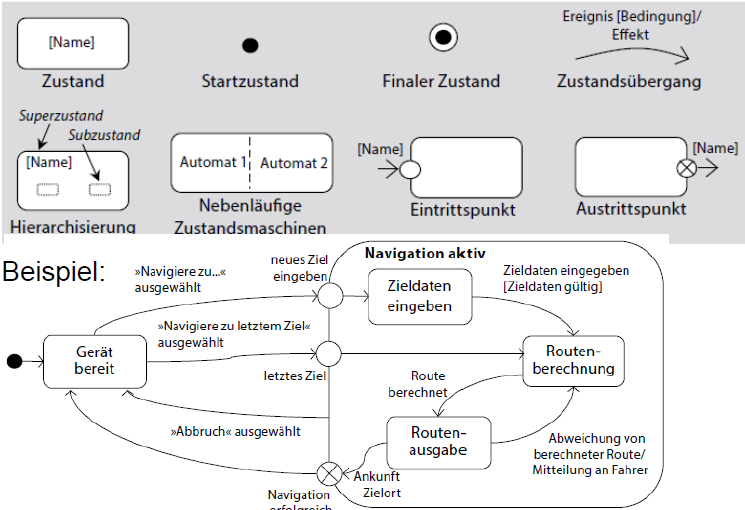
\includegraphics[width=150px]{img/UMLZustandsdiagram.png}
        \captionof{figure}{Elemente des UML Zustandsdiagram}
        \label{fig:Elemente des UML Zustandsdiagram}
\end{Figure}

\section{Dokumentation im agilen Umfeld}
Recap: Wie funktioniert Scrum
\begin{Figure}
   \centering
    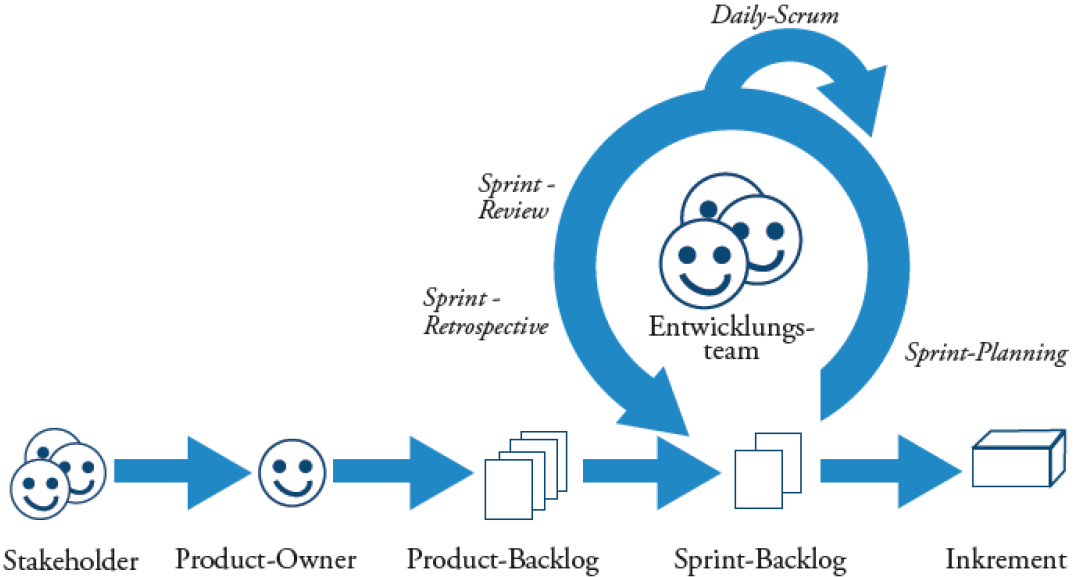
\includegraphics[width=150px]{img/Scrum.png}
        \captionof{figure}{Überblick Vorgehen nach Scrum}
        \label{fig:Vorgehen nach Scrum}
\end{Figure}

\begin{itemize}
   \item Normalerweise werden in einem Sprint alle Tätigkeiten zur Entwicklung (inkl. Analyse) des Inkrements durchgeführt, um die erforderlichen Informationen genau zu dem Zeitpunkt zu erzeugen, zu dem sie auch benötigt werden
   \item Je nach Domäne und Projektrandbedingungen muss aber auch schon vorher und nachher noch RE betrieben werden
   \item Product Owner und Entwicklungsteam benötigen Tätigkeiten aus verschiedenen RE-Disziplinen für ihren Aufgabenbereich
   \item Die Auswahl der einzelnen Techniken in diesen Tätigkeiten kann sich zum Teil in einem Projekt immer wieder ändern, da sie sehr stark von den aktuellen Gegebenheiten abhängen
   \item Die Verantwortlichkeit für die Auswahl dem Entwicklungsteam zu überlassen, kommt diesem Umstand sehr entgegen, da sie am besten die aktuell vorliegende Situation einschätzen und so die optimale Auswahl treffen können
   \item Für jeden Typ von Informationen, der zur Dokumentation ansteht, sind folgende Fragen zu stellen
   \subitem \textit{Wie} lange nach der Entstehung wird die Information benötigt?
   \subitem \textit{Wann} soll die Information dokumentiert werden?
   \subitem \textit{Wie} soll dokumentiert werden? 
\end{itemize}

\begin{Figure}
   \centering
    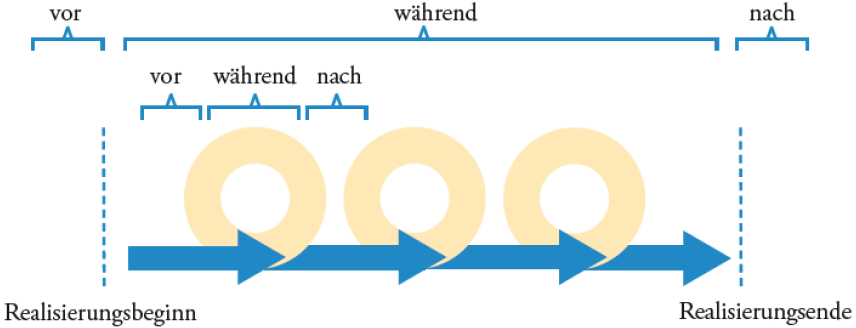
\includegraphics[width=150px]{img/ScrumOptionen.png}
        \captionof{figure}{Integrations-Optionen von RE in Scrum}
        \label{fig:Integrations-Optionen von RE in Scrum}
\end{Figure}

\subsection{User Stories}
\begin{itemize}
   \item Eine User Story beschreibt eine Funktionalität, die für den Kunden oder Benutzer eines Produkts oder Systems von Wert ist
   \item Sie besteht aus der schriftlichen Beschreibung der Funktionalität, Gesprächen über die Funktionalität und Akzeptanzkriterien, die Details vermitteln und festlegen, wann eine User Story vollständig umgesetzt ist
   \item $\Rightarrow$ eine User Story ist in einem Sprint durchzuführen, entsprechend muss man diese 'abschneiden'
   \item Akzeptanzkriterien legen fest, unter welchen Bedingungen ein Product-Backlog-Eintrag (bspw. User Story) als umgesetzt gilt und erfolgreich abgenommen wird
\end{itemize}

\subsection{Technical Stories}
\begin{itemize}
   \item Beschreiben keine Funktionalität $\rightarrow$ werden oft als Technical Stories bezeichnet
   \item umfassen technische oder andere nicht-funktionalite Aspekte, die nicht über die Implementierung einzelner User Stories abgedeckt werden (bspw. Refactoring)
\end{itemize}

\subsection{Definition of Done (DoD)}
$\rightarrow$ man eignet sich im Team \textit{Wann ist man fertig}
\begin{itemize}
   \item Die Definition of Done bezieht sich immer auf das Ergebnis eines Entwicklungszyklus
   \item Kann bei Bedarf angepasst werden
   \item Der Scrum-Guide definiert die DoD als ein Artefakt, das bei allen Projektbeteiligten ein gemeinsames Verständnis dafür erzeugt, welche formalen Kriterien erfüllt sein müssen, damit die Arbeit an einem System- oder Produktinkrement als abgeschlossen gilt
\end{itemize}

\begin{Figure}
   \centering
    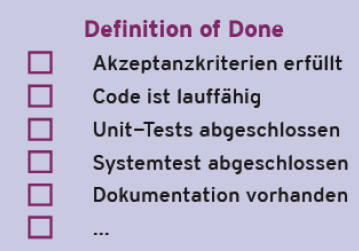
\includegraphics[width=150px]{img/DoD.png}
        \captionof{figure}{Beispiel DoD}
        \label{fig:Beispiel DoD}
\end{Figure}

\subsection{Story Maps}

\begin{itemize}
   \item Use Cases und User Stories haben eine ähnliche Ausrichtung:
   \subitem bilden einzelne Systemfunktionalitäten aus der Sicht eines Benutzers ab
   \subitem liefern Übersicht über das System
   \subitem Use Cases sind jedoch überlicherweise auf gröberer Ebene als User Stories
   \subitem Ein Use Case umfasst mehrere oder sogar viele User Stories
   \subitem Epic wiederum kann in seinem Umfang einem groben Use Case entsprechen
   \item Dokumentationstechniken von Use Cases können auch auf User Stories übertragen werden
   \item User Stories vs. Use Cases
   \subitem Es werden nur jene ANforderungen im Detail ausgearbeitet, die in kommenden Iterationen realisiert werden $\rightarrow$ User Stories unterstützen diesen Prozess
   \subitem Funktionen welche erst später geplant sind, werden zunächst nur grob aufgenommen
   \subitem User Stories alleine eignene sich hingege nicht besonders gut dazu, das Wissen über Anforderungen langfristig aufzubewahren, sofern dies notwendig und angebracht ist
   \subitem Die Dokumentation mittels Use Cases, das Festhalten von Entscheidungen, Szenarien mit ergänzenden Kontextinformationen usw. sind dazu besser geeignet 
\end{itemize}

\begin{Figure}
   \centering
    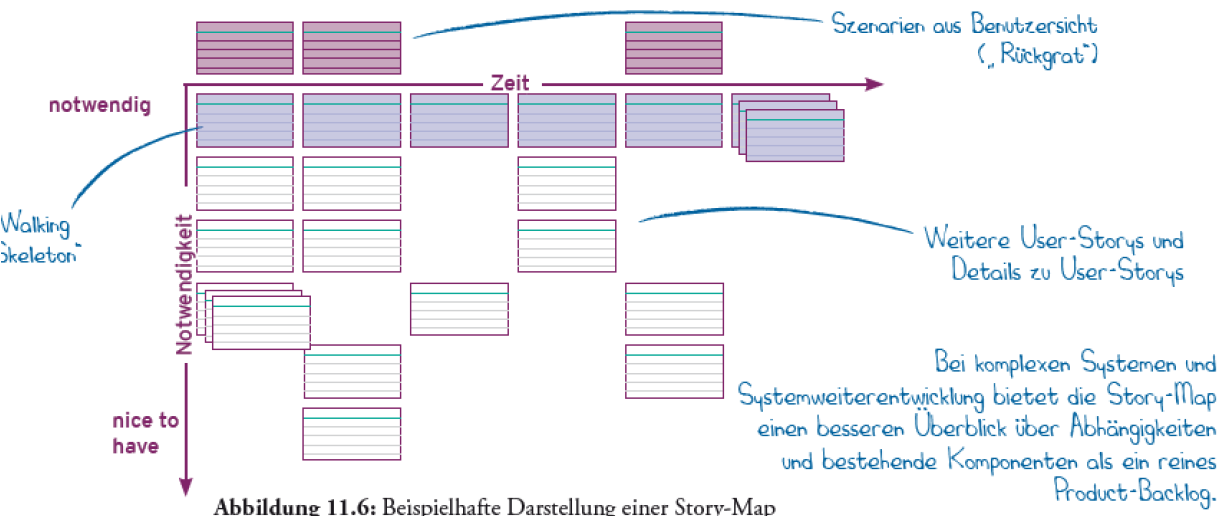
\includegraphics[width=150px]{img/StoryMap.png}
        \captionof{figure}{Beispiel einer StoryMap}
        \label{fig:Beispiel einer StoryMap}
\end{Figure}

\begin{Figure}
   \centering
    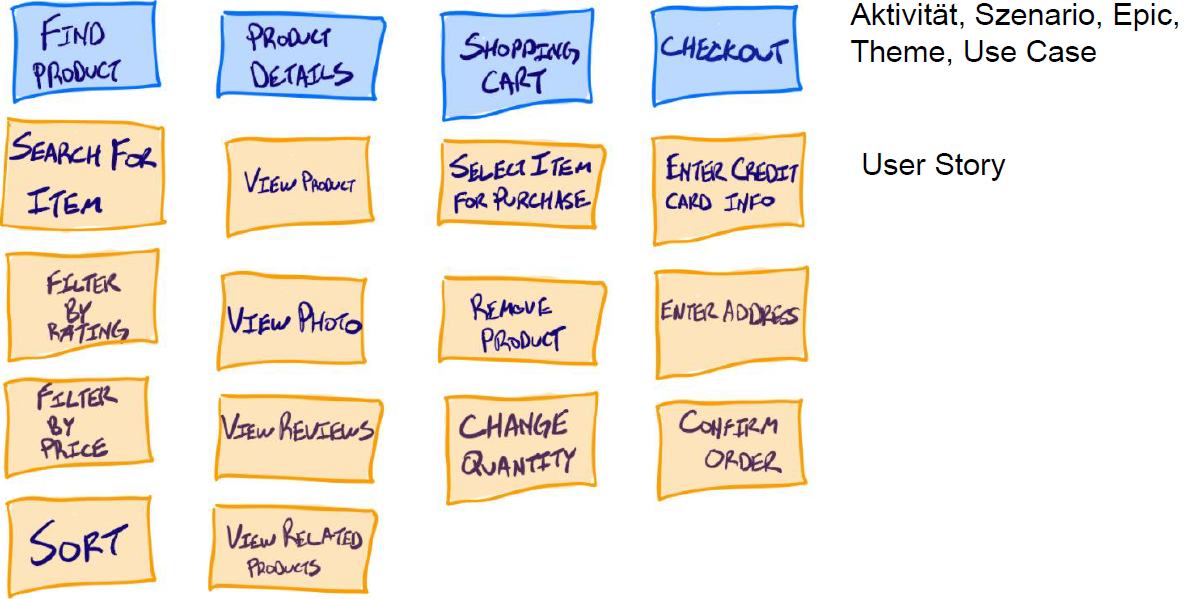
\includegraphics[width=150px]{img/StoryMappII.png}
        \captionof{figure}{Beispiel einer weiteren StoryMap}
        \label{fig:Beispiel einer weiteren StoryMap}
\end{Figure}

\section{Anforderungen prüfen und abstimmen}
Die Zielsetzung der Prüfung von Anforderungen besteht darin, Anforderungen dahingehend zu überprüfen, ob sie festgelegten Qualitätskriterien (bspw. Korrektheit oder Vollständigkeit) genügen, um etwaige Fehler in den Anforderungen möglichst frühzeitig im RE erkennen und beheben zu können.

\subsection{Grundlage}
\begin{itemize}
   \item Ziel: Auffinden von Fehlern $\rightarrow$ bspw. Mehrdeutigkeit, Unverständlichkeit, Widersprüche
   \item Anforderungsdokumente sind die Grundlagen
   \item Fehler beeinträchtigen alle weiteren Entwicklungstätigkeiten
   \item Fehlerfortpflanzung: nicht nur die Anforderung muss angepasst werden, sondern allenfalls auch Architektur, Artefakten etc.
   \item Freigabe von Anforderungen
   \item Verträge zwischen Auftraggeber und Auftragnehmen basieren oft auch auf Anforderungsdokumenten
\end{itemize}
\textbf{ABstimmung von Anforderungen}
\begin{itemize}
   \item Ziel der Abstimmung von Anforderungen ist es, unter den relevanten Stakeholder ein gemeinsames und übereinstimmendes Verständnis hinsichtlich der Anforderungen an das zu entwickelnde System zu erarbeiten
   \item Wiedersprechende Anforderungen erzeugen Konflikte
   \item Risiken und Chancen: die AKzeptanzt eines geplanten Systems wird durch unaufgelöste Konflikte gefährdet
\end{itemize}

\subsection{Qualitätsaspekte}
\begin{itemize}
   \item Inhalt
   \item Dokumentation
   \item Abgestimmtheit
\end{itemize}

\subsubsection{Prüfen des Inhalts}
Ziel: Vermeiden, dass die Entwicklung auf falscher Information basiert, d.h. entwickelt wird, was nicht benötigt wird.\\
Gesucht werden Mängel im Bezug auf
\begin{itemize}
   \item Vollständigkeit $\rightarrow$ Alle Bedürfnisse umgesetzt / beschrieben
   \item Verfolgbarkeit $\rightarrow$ Identifikation und Quellen
   \item Korrektheit / Adäquatheit
   \item Konsistenz $\rightarrow$ keine Widersprüche
   \item Keine vorzeitigen Entwurfsentscheidungen
   \item Überprüfbarkeit $\rightarrow$ Abnahmekriterium möglich
   \item Notwendigkeit $\rightarrow$ Trägt zu einem Ziel bei
\end{itemize}

\subsubsection{Prüfen der Dokumentation}
Ziel: Vermeiden, dass Information fehlt oder nicht gemäss geforderten oder vereinbarten Erfordernissen aufbereitet ist\\
Gesucht werden Mängel im Bezug auf
\begin{itemize}
   \item Konformität
   \item Verständlichkeit
   \item Eindeutigkeit
\end{itemize}

\subsubsection{Prüfen der Abgestimmtheit}
Ziel: Vermeiden, dass nicht alle Stakeholder mit den dokumentierten Anforderungen übereinstimmen\\
Gesucht werden Mängel im Bezug auf
\begin{itemize}
   \item Abstimmung
   \item Abstimmung Änderungen
   \item Konflikte
\end{itemize}

\subsection{Prinzipen der Prüfung von Anforderungen}
\begin{enumerate}
   \item Die richtigen Stakeholder beteiligen
   \item Fehlersuche und Fehlerkorrektur trennen
   \item Aus unterschiedlichen Sichten prüfen
   \item Dokumentationsform geeignet wechseln
   \item Entwicklungsartefakte konstruieren
   \item Prüfung wiederholen
\end{enumerate}

\subsection{Techniken zur Prüfung von Anforderungen}
Für die systematische Prüfung von Anforderungen existieren versch. Techniken, die teilweise auch ergänzend zueinander eingesetzt werden, um Anforderungen möglichst umfassend hinsichtlich festgelegter Prüfkriterien zu überprüfen.
\begin{itemize}
   \item Stellungsnahme
   \item Inspektion
   \item Walkthrough
   \item Perspektivenbasiertes Lesen
   \item Prüfung durch Prototypen
   \item Einsatz von Checklisten
\end{itemize}

\subsubsection{Stellungsnahme}
Ziel: dritte Person erstellt eine Expertise bezüglich Qualität
\begin{itemize}
   \item Der Autor übergibt seine Anforderungen an eine dritte Person
   \item Identifikation von Qualitätsmängel /Mehrdeutigkeit und Fehler
\end{itemize}

\subsubsection{Inspektion}
$\rightarrow$ Ist ein sehr formaler Prozess
\begin{itemize}
   \item Inspektionen haben das Ziel, Entwicklungsartefakte systematisch nach Fehlern zu durchsuchen
   \item Eine Inspektion besteht aus den Phasen
   \subitem Planung
   \subitem Übersicht
   \subitem Fehlersuche
   \subitem Fehlersammlung
   \subitem Nachkontrolle
   \subitem Reflexion
\end{itemize}

Dabei kommen unterschiedliche Rollen zum Zug:
\begin{itemize}
   \item Moderator
   \item Organisator
   \item Autor
   \item Vorleser
   \item Inspektoren
   \item Protokollführer
\end{itemize}

$\Rightarrow$ als Output resultiert ein \textbf{Review-Bericht}

\subsubsection{Walkthrough}
$\rightarrow$ leichtgewichtiges Review / Inspektion

\begin{itemize}
   \item Weniger Strikt
   \item Drei Rollen
   \subitem Reviewer
   \subitem Autor
   \subitem Protokollant
\end{itemize}

\subsubsection{Perspektivenbasiertes Lesen}
$\rightarrow$ Lesen aus unterschiedlichen Perspektiven
\begin{itemize}
   \item Perspektiven Kunden/Nutzer
   \item Perspektive Softwarearchitektur
   \item Perspektive Tester
\end{itemize}
oder alternativ aus den Perspektiven
\begin{itemize}
   \item Perspektive Inhalt
   \item Perspektive Dokumentation
   \item Perspektive Abgestimmtheit
\end{itemize}

\subsubsection{Prüfung durch Prototypen}
\begin{itemize}
   \item Die Prüfung von Anforderungen durch Prototypen verfolgt den Ansatz, die Anforderungen für den Prüfer erlebbar und damit ausprobierbar zu machen
   \subitem Wegwerfprototypen $\rightarrow$ wird anschliessend weggeworfen
   \subitem Evolutionäre Prototyp $\rightarrow$ dieser Protoypen wächst weiter
   \item Vor der Prüfung muss festgelegt werden, welcher Anforderungen mit dem Prototypen überprüft werden sollen
   \item Vorbereitung
   \subitem Handbuch / Schulung
   \subitem Prüfszenarien
   \subitem Checklisten mit Prüfkriterien
   \item Prüfung der Anforderungen durch Prototypen kann wie folgt dokumentiert werden
   \subitem Protokoll des Prüfers
   \subitem Beobachtungsprotokoll (durch eine zweite Person)  
\end{itemize}

\subsubsection{Einsatz von Checklisten}
\begin{itemize}
   \item tbd ...
\end{itemize}


\subsection{Abstimmung von Anforderungen}
Die Abstimmung von Anforderungen zielt darauf ab, ein gemeinsames Verständnis der Anforderungen andas zu entwickelnde System unte rallen relevanten Stakeholder herzustellen.\\
Dabei gibt es folgende Aufgaben
\begin{itemize}
   \item Konfliktidentifikation
   \item Konfliktanalyse
   \item Konfilktauflösung
   \item Dokumentation von Konfliktlösungen
\end{itemize}

\subsubsection{Konfliktanalyse}
$\rightarrow$ ein identifizierter Konflikt wird auf seine Ursache untersucht\\
Dabei gibt es unterschiedliche Konflikttypen:
\begin{itemize}
   \item Sachkonflikt $\rightarrow$ Mangel an Informationen oder Fehlinformationen
   \item Interessenskonflikt $\rightarrow$ geringe Kosten vs. hohe Qualität
   \item Wertekonflikt $\rightarrow$ kulturelle Unterschiede
   \item Beziehungskonflikt $\rightarrow$ Emotionen. schlechte Kommunikation
   \item Strukturkonflikt $\rightarrow$ ungleiche Macht und Autoritätsverhältnisse
\end{itemize}

\subsubsection{Konfliktauflösung}
$\rightarrow$ alle Stakeholder müssen miteinbezogen werden.\\

Dabei gibt es folgende Konfliktlösungstechniken:
\begin{itemize}
   \item Einigung $\rightarrow$ durch Austausch von Informationen 
   \item Kompromisse $\rightarrow$ Kombination aus Lösungsalternativen
   \item Abstimmung $\rightarrow$ es wird über Alternativen abgestimmt
   \item Variantebildung $\rightarrow$ durch Variantenauswahl oder Parametrierung versch. Systemvarianten
   \item Ober-sticht-Unter $\rightarrow$ ranghöhrere Partei entscheidet
   \item Consider all Facts $\rightarrow$ untersuchen aller Einflussfaktoren, Priorisierung, Relevanz
   \item Plus Minus Interesting $\rightarrow$ Positive Negative Auswirkungen der Lösungsvarianten
   \item Entscheidungsmatrix $\rightarrow$ Nutzwerkanalyse, evtl. mit Gewichtung
   \subitem Wenn sich die Lösungsvarianten nur sehr marginal in der Punktzahl unterscheiden, müssen unbedingt eine Sensibilitätsanalyse durchgeführt werden und evtl. weitere Techniken zur Konfliktauflösung eingesetzt werden 
\end{itemize}

\begin{Figure}
   \centering
    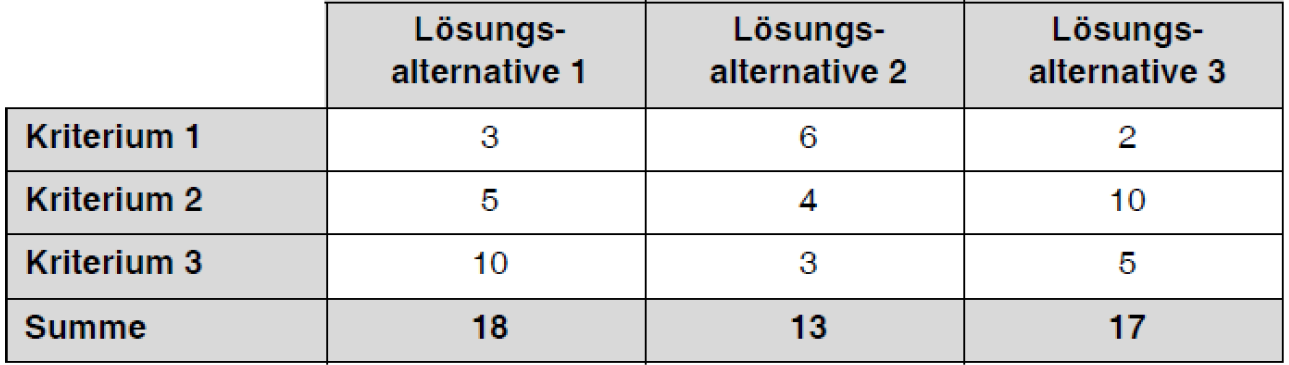
\includegraphics[width=150px]{img/Entscheidungsmatrix.png}
        \captionof{figure}{Beispiel einer Entscheidungsmatrix}
        \label{fig:Beispiel einer Entscheidungsmatrix}
\end{Figure}


\section{Anforderungen verwalten}
Anforderungen verwalten gehört zu einer der vier Haupttätigkeiten im RE.

\subsection{Attribute von Anforderungen}
\textbf{Grundsatz:} Um die Anforderungen an ein System über den gesamten Lebenszyklus des Systems hinweg verwalten zu können, ist es notwendig die Informationen zur Anforderung als Attribute möglichst strukturiert zu erfassen.

\subsubsection{Attributierungsschema}
Die Definition der Attributstruktur für Anforderungen erfolgt über ein Attributierungsschema, das entweder tabellarisch oder in Form eines Informationsmodells definiert werden kann\\

einige typische Attributstypen werden nachfolgend aufgelistet:

\begin{Figure}
   \centering
    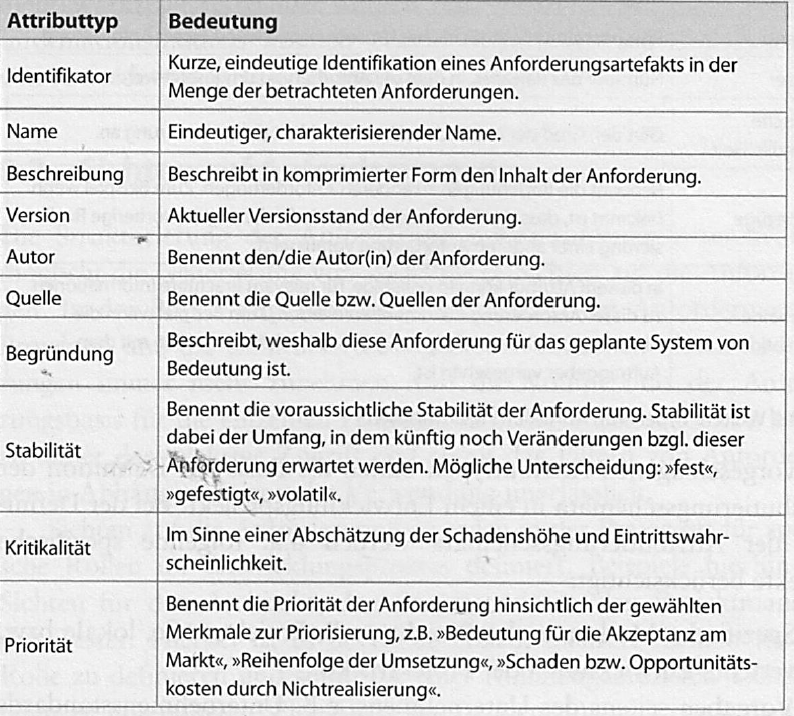
\includegraphics[width=150px]{img/AttributeI.png}
        \captionof{figure}{Beispiel gewisser Attributtypen I}
        \label{fig:Beispiel gewisser Attributtypen I}
\end{Figure}

\begin{Figure}
   \centering
    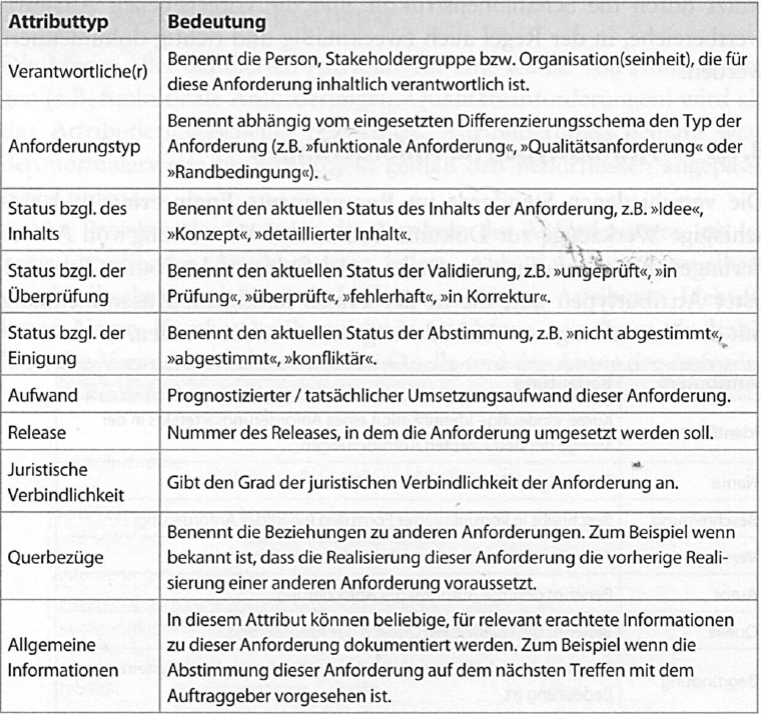
\includegraphics[width=150px]{img/AttributeII.png}
        \captionof{figure}{Beispiel gewisser Attributtypen II}
        \label{fig:Beispiel gewisser Attributtypen II}
\end{Figure}

$\Rightarrow$ Attributierungsschema werden dabei häufig projektspezifisch auf Basis bestimmter Rahmenbedingungen definiert bzw. angepasst. \\
Hierzu gehören:
\begin{itemize}
   \item Spezifische Merkmale
   \item Vorgaben
   \item Vorschriften
   \item Randbedingungen
\end{itemize}


\subsection{Sichten auf Anforderungen}
Sichten sind ein reduzierter Zugriff auf die relevanten Anforderungen bspw. nur für bestimmte Rollen oder Personen relevant. \\
Dabei unterscheiden wir zwischen:
\begin{itemize}
   \item Selektive Sichten $\rightarrow$ Darstellung einer Teilmenge der Attributwerte von über definierte Selektionskriterien ausgewählten Anforderungen $\Rightarrow$ für spezifische Rolle
   \item Verdichtende Sichten $\rightarrow$ Darstellung verdichteteter Informationen zu den über definierte Selektionskriterien ausgewählten Anforderungen $\Rightarrow$ Auswertung
\end{itemize}

\subsection{Priorisierung von Anforderungen}
Anforderungen werden zu versch. Zeitpunkten in versch. Aktivitäten nach unterschiedlichen Kriterien priorisiert

\subsubsection{Vorgehen}
Die Vorbereitung der Priorisierung von Anforderungen basiert auf einer einfachen Systematik:
\begin{itemize}
   \item Bestimmung der Ziele und Randbedingungen der Priorisierung
   \item Bestimmung der Priorisierungskriterien (Kosten, Risiko, Schaden bei nicht Erfolg, Volatiltiät, Wichtigkeit)
   \item Bestimmung der relevanten Stakeholder
   \item Auswahl der zu priorisierende Artefakte
\end{itemize}

\subsubsection{Techniken}
Es gibt verschiedene Techniken zur Priorisierung.
\begin{enumerate}
   \item \textbf{Ranking} $\rightarrow$ Rangfolge von Anforderungen wird von ausgewählten Stakeholder ausgewählt
      \subitem in der Praxis haben relativ schnell, alle Anforderungen Prio 1 erhalten
      \subitem Man kann den Stakeholder dazu 'zwingen' die Anforderungen in ein Ranking zu verpacken 
   \item \textbf{Top-Ten Technik} $\rightarrow$ Für ein betrachtetets Kriterium werden die $n$ wichtigsten Anforderungen ausgewählt
   \item \textbf{Ein-Kriterium-Klassifikation} $\rightarrow$ basiert auf der Wichtigkeit der Realisierung
      \subitem nach IEEE-830-1998 drei Prioritätsklassen
         \subsubitem Mandatory
         \subsubitem Optional
         \subsubitem nice-to-have
   \item \textbf{Kano-Klassifizierung} $\rightarrow$ Analog dem Kano-Modell
      \subitem Klassifizierung in 
         \subsubitem Basismerkmale
         \subsubitem Leistungsmerkmale
         \subsubitem Begeisterungsmerkmale
   \item Wiegers'sche Priorisierungsmatrix $\rightarrow$ sehr aufwändig, wird nicht weiter betrachtet
\end{enumerate}

\subsection{Verfolgbarkeit von Anforderungen}
Im Rahmen der Verwaltung von Anforderungen werden Verfolgbarkeitsinformationen von Anforderungen aufgezeichnet, organisiert und gepflegt und dies über den gesamten Lifecycle\\
\textbf{Definition:} Information auf der Basis eines klar definierten Verwendungszweckes und wird später in der Systementwicklung oder Systemevolution gebraucht

\subsubsection{Nutzen}
\begin{itemize}
   \item Vereinfachung der Nachweisbarkeit
   \item Identifikation von unnötigen Eigenschaften im System
   \item Identifikation von unnötigen Anforderungen
   \item Unterstützung der Auswirkungsanalyse ($\rightarrow$ Entwicklungsartefakte)
   \item Unterstützung der Wiederverwendung
   \item Unterstützung der Festlegung der Zurechenbarkeit (Zuordnung des Aufwandes, Nachkalkulation)
   \item Unterstützung der Wartung und Pflege
\end{itemize}

\subsubsection{Klassifikation von Verfolgbarkeitsbeziehungen}
hinsichtlich der Verfolgbarkeitsbeziehungen von Anforderungen werden drei Klassen von Verfolgbarkeitsbeziehungen unterschieden:
\begin{itemize}
   \item Pre-Requirements-Specification-Traceability
   \item Post-Requirements-Specification-Traceability
   \item Traceability zwischen Anforderungen
\end{itemize}

\begin{Figure}
   \centering
    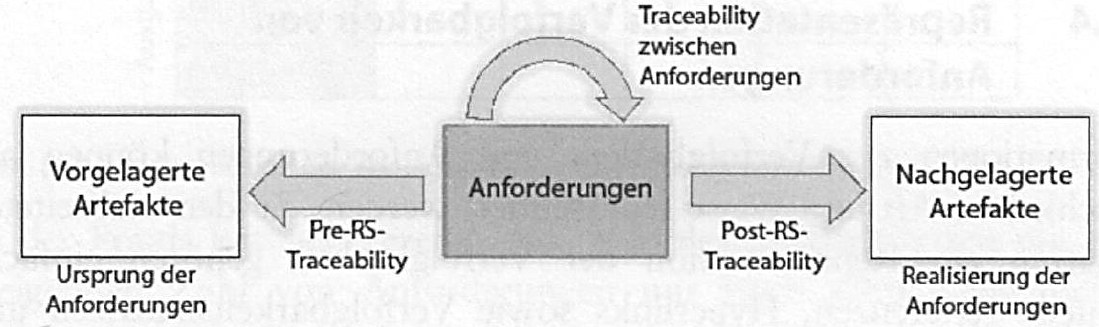
\includegraphics[width=150px]{img/KlassifikationTraceability.png}
        \captionof{figure}{Abbildung der Klassen der Traceability}
        \label{fig:Abbildung der Klassen der Traceability}
\end{Figure}

\subsection{Versionierung von Anforderungen}
Die Versionierung und Konfiguration von Anforderungen ermöglicht es, über den Lebenszyklus eines Systems oder Produktes hinwes, spezfische Entwicklugnsstände (von Anforderungen und Anforderungsdokumenten) verfügbar zu halten.

\subsubsection{Konfiguration von Anforderungen}
Eine Anforderungskonfiguration fasst eine definierte Menge logisch zusammengehöriger Anforderungen zusammen, wobei jede Anforderung maximal in einer Version in der Anforderungskonfiguration enthalten ist. Dabei unterscheidet man zwischen zwei Dimensionen:
\begin{itemize}
   \item Produktdimension: die einzelnen Anforderungen der Anforderungsbasis
   \item Versionsdimension: die versch. Versionsstände einer Anforderungen
\end{itemize}

\subsubsection{Anforderungsbasislinien}
Anforderungsbasislinien sind ausgezeichnete Anforderungskonfigurationen, die stabile Versionen von Anfroderungen umfassen und oftmals auch Auslieferungsstufen des Systems definiernen
\begin{itemize}
   \item Grundlage zur Planung von Auslieferungsstufen
   \item Abschätzung des Realisierungsaufwandes
   \item Vergleichen mit Konkurrenzprodukten
\end{itemize}

\subsection{Verwaltung von Anforderungsänderungen}
Über den gesamten Lebenszyklus eines Systems hinweg verändern sich die Anfroderungen. Die Änderungen an en Anfroderungen werden in einem systematischen Änderungsmanagementprozess verwaltet und bearbeitet

\subsubsection{Change Control Board}
Im Änderungsmanagementprozess ist das Change-Control-Board (CCB) für die Bearbeitung eingehender Änderungsanträge verantwortlich. \\
Die Aufgaben des CCB sind:
\begin{itemize}
   \item Klassfikation eingehender Änderungsanträge
   \item Bestimmung des Aufwands einer Änderung
   \item Beurteilung der Änderungsanträge hinsichtlich Aufwand / Nutzen
   \item Definition neuer Anforderungen auf Basis eingehender Änderungsanträge
   \item Entscheidung über Annahme oder Ablehnung eines Änderungsantrags
   \item Priorisierung der agenommene Änderungsanträge
   \item Zuordnung der Änderungen zu Änderungsprojekten
\end{itemize}

Typische Vertreter sind:
\begin{itemize}
   \item Änderungsmanager 
   \item Auftraggeber
   \item Architekt
   \item Nutzervertreter
   \item Qualitätsbeauftragter
   \item Anforderungsingenieur
\end{itemize}

\subsubsection{Änderungsantrag}
Für notwendig erachtet Änderungen von Anforderungen werden in Form von Änderungsanträgen dokumentiert und an das CCB übermittelt.\\
Dabei umfasst der Antrag mind. folgende Informationen:
\begin{itemize}
   \item Identifikator des Änderungsantrags
   \item Titel 
   \item Beschreibung der notwendigen Änderung
   \item Begründung
   \item Datum
   \item Antragssteller
   \item Priorität
   \item Zusätzliche Informationen
   \subitem Prüfer der Änderung
   \subitem Status der Auswirkungsanalyse
   \subitem Status der Entscheidung CCB
   \subitem Priorität CCB
   \subitem Verantwortlicher für Umsetzung
   \subitem Systemrelease
\end{itemize}

\subsubsection{Klassifikation}
Drei Arten eines Änderungsantrags
\begin{itemize}
   \item Korrektive Änderungen $\rightarrow$ Fehlverhalten
   \item Adaptive Änderungen $\rightarrow$ Anpassung des Systems
   \item Ausnahmeänderungen $\rightarrow$ Hotfix, muss unmittelbar umgesetzt werden
\end{itemize}

Dabei sieht das Vorgehen für korrektive und adaptive Änderungen wie folgt aus:
\begin{itemize}
   \item Auswirkungsanalyse und Beurteilung der Änderung
   \item Priorisierung der Anforderungsänderung
   \item Zuordnung der Änderung zu einem Änderungsprojekt
   \item Kommunikation der Annahme / Ablehnung des Änderungsantrages
\end{itemize}

\section{Werkzeugunterstützung}

\subsection{Allgemeine Werkzeugunterstützung}
Viele Systementwicklungswerkzeuge können auch RE unterstützen
\begin{itemize}
   \item Testverwaltungswerkzeuge
   \item Konfigurationswerkzeuge
   \item Wiki
   \item Bürosoftware Visualisierungswerkzeuge
\end{itemize}

\subsection{Modellierungswerkzeuge}
Tool-Suiten
\begin{itemize}
   \item UML / BPMN / TOGAF: Enterprise Architect (Sparx)
   \item IMB Rational Tool Suite
   \item Magic draw
   \item \dots
\end{itemize}

Features
\begin{itemize}
   \item UML Modellierung
   \item Model Driven Architecture (MDA)
   \item Reverse Engineering
   \item Standard Schnittstellen
   \item \dots
\end{itemize}

\subsection{Requirements-Management-Werkzeuge}
Ein Requirements-Management-Werkzeug sollte dabei folgende grundlegende Eigenschaften aufweisen
\begin{itemize}
   \item Verschiedene Informationen verwalten
   \item logische Beziehungen zwischen Informationen verwalten
   \item Jdes Artefakt eindeutig identifizieren
   \item Informationen flexibel und sicher zugänglich machen, bspw. durch Zugriffskontrolle
   \item Sichten auf die Informationen unterstützen
   \item Informationen organisieren bspw. durch Attributierung und Hierarchiebildung
   \item Berichte über die Informationen erstellen
   \item DOkumente aus den Informationen generieren
\end{itemize}

Spezialisierte Requirements-Management-Werkzeuge (bspw. IBM Rational RequistitePro bzw. IBM Rational DOORS)\\
Charakteristische Eigenschaften dieser Werkzeuge sind:
\begin{itemize}
   \item Verwaltung von Anforderungen und Attributen auf der Basis von Informationsmodellen
   \item Organisation von Anforderungen (mittels Hierarchieebenen)
   \item Konfigurations- und Versionsmanagement auf Anforderungsebene
   \item Definition von Anforderungsbasislinien
   \item Mehrbenutzerzugriff und -verwaltung (bspw. Zugriffskontrolle)
   \item Verfolgbarkeitsmgmt (Traceability Management)
   \item Konsolidierung der erfassten Anforderungen (bspw. Sichtenbildung)
   \item Unterstützung des Änderungsmanagement (Änderungskontrolle)
\end{itemize}

\subsection{Werkzeugeinführung}
Erst nach der Einführung von RE-Vorgehensweise und Techniken kann ein passendes Werkzeug ausgesucht werden. Diese Einführung setzt klare Verantwortlichkeiten und Vorgehensweise im RE voraus. Dabei sind folgende Gesichtspunkte zu beachten:
\begin{itemize}
   \item Benötigte Ressourcen planen
   \item Risiken durch Pilotprojekte umgehen
   \item Evaluierung anhand von definierten Kriterien
   \item Über Lizenzkosten hinausgehende Kosten berücksichtigen
   \item Benutzer schulen
\end{itemize}

\subsection{Beurteilung von Werkzeugen}
Die Bewertung lässt sich auf sieben Sichten strukturieren
\begin{itemize}
   \item Projektsicht $\rightarrow$ Unterstützung der Projektplanung
   \item Benutzersicht $\rightarrow$ insbesondere Bedienung
   \item Produktsicht $\rightarrow$ Funktionalität
   \item Prozesssicht $\rightarrow$ methodische Unterstützung
   \item Anbietersicht $\rightarrow$ Service des Anbieters
   \item Technische Sicht $\rightarrow$ Interoperabiltität, Skalierbarkeit
   \item betriebwirtschaftliche Sicht $\rightarrow$ Kosten
\end{itemize}
$\Rightarrow$ Für jede Sicht sind klare Kriterien zu definieren



\chapter{Software Architektur}
Es gibt durchaus parallelen zur klassischen Architektur $\rightarrow$ gute Architektur:\\
\begin{itemize}
   \item utilitas (Nützlichkeit)
   \subitem Die Software erfüllt die \textbf{funktionalen und nicht-funktionalen Anforderungen} der Nutzer und Kunden  
   \item firmitas (Festigkeit)
   \subitem Die Software ist stabil im Hinblick auf die \textbf{geforderten Qualitätseigenschaften} z.B. langlebig, da zukünftige Weiterentwicklungen möglich sind, ohne das System komplett neu zu bauen 
   \item venustas (Schönheit)
   \subitem Die Software ist sowohl \textbf{aussen} (gegenüber dem Nutzer) wohl strukturiert, sodass sie inuitiv nutzbar ist, als auch \textbf{innen} (gegenüber demjenigen, der die Software pflegen und weiterentwicklen soll) wohl strukturiert, sodass dieser die internen Strukturen der Software leicht verstehen und damit gut seinen Aufgaben nachkommen kann
\end{itemize}


\section{Grundlagen}
Der CHOAS-Report der Standisch Group zeigt, dass wir es immer noch nicht schaffen, wiederholbar qualitativ \textbf{hochwertige Software} zu erschwinglichen \textbf{Kosten} und im vorgegeben Zeitfenster mit der notwendigen \textbf{Funktionalität}

\begin{Figure}
   \centering
    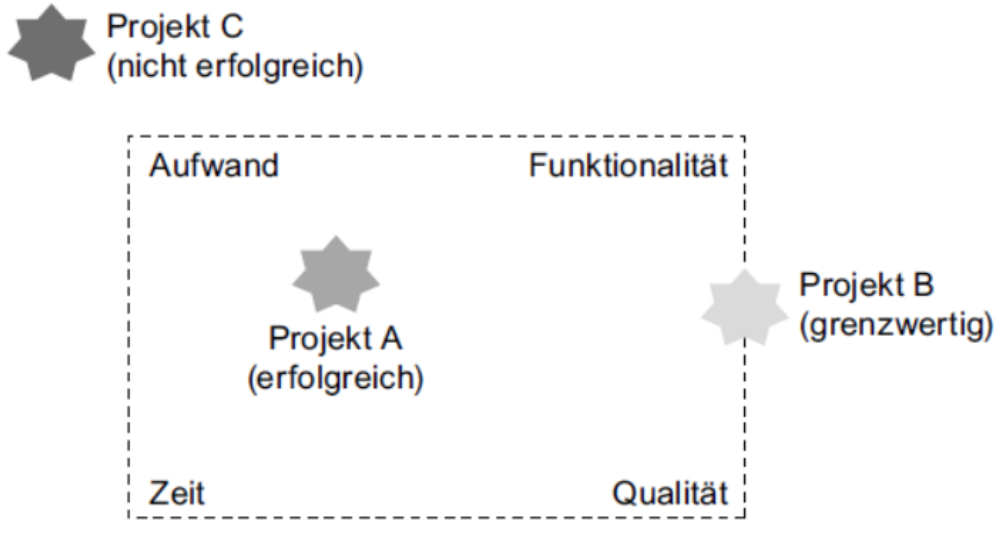
\includegraphics[width=150px]{img/chaosReport.png}
        \captionof{figure}{Abbildung des magischen Dreiecks zwischen Aufwand, Zeit, Funktionen, Qualitaet}
        \label{fig:Abbildung des magischen Dreiecks zwischen Aufwand, Zeit, Funktionen, Qualitaet}
\end{Figure}


\subsection{Definitionen}
\textbf{Was ist Softwarearchitektur?}
\begin{itemize}
   \item RE und Architekturentwurf zwei zentrale Schlüsselfaktoren
   \item Bei beiden ist das Risiko von gravierenden Fehlentwicklung hoch
\end{itemize}

\textbf{System:} \textit{A collection of components organized to accomplish a specific funcion or set of functions}\\
\textbf{Software:} \textit{Computer programs, procedures, and possibly associated documentation and data pertaining to the operation of acomputer system}\\
\textbf{Softwareintensives System}
\begin{itemize}
   \item Menge von Bausteinen
   \item Bausteine, die aus Software bestehen übernehmen wesentliche Aufgaben zur Erfüllung des Systemszweck
\end{itemize}

\textbf{Softwarearchitektur}: Die Softwarearchitektur definiert die grundlegenden Prinzipien und
Regeln für die Organisation eines Systems sowie dessen
Strukturierung in Bausteinen und Schnittstellen und deren
Beziehungen zueinander wie auch zur Umgebung. Dadurch legt sie
Richtlinien für den gesamten Systemlebenszyklus, angefangen bei
Analyse über Entwurf und Implementierung bis zu Betrieb und
Weiterentwicklung, wie auch für die Entwicklungs- und
Betriebsorganisation fest.\\

\textbf{Schnittstelle:}
\begin{itemize}
   \item repräsentiert einen wohldefinierten Zugangspunkt zum System oder dessen Bausteinen
   \item Beschreibt Eigenschaften dieses Zugangspunkts (bspw. Attribute, Daten und Funktionen)
\end{itemize}

\subsection{Grundlegende Konzepte}
\begin{itemize}
   \item Es ist eine Art Bauplan für die Festlegung der Struktur und Konzepten
   \item Hierarchische Zerlegung in eine Menge von Bestandteilen
\end{itemize}

\subsection{Bausteine}
Beinhaltet sämtliche Software- oder Implementierungsartefakte, die letztendlich Abstraktionen von Quellcode darstellen
\begin{Figure}
   \centering
    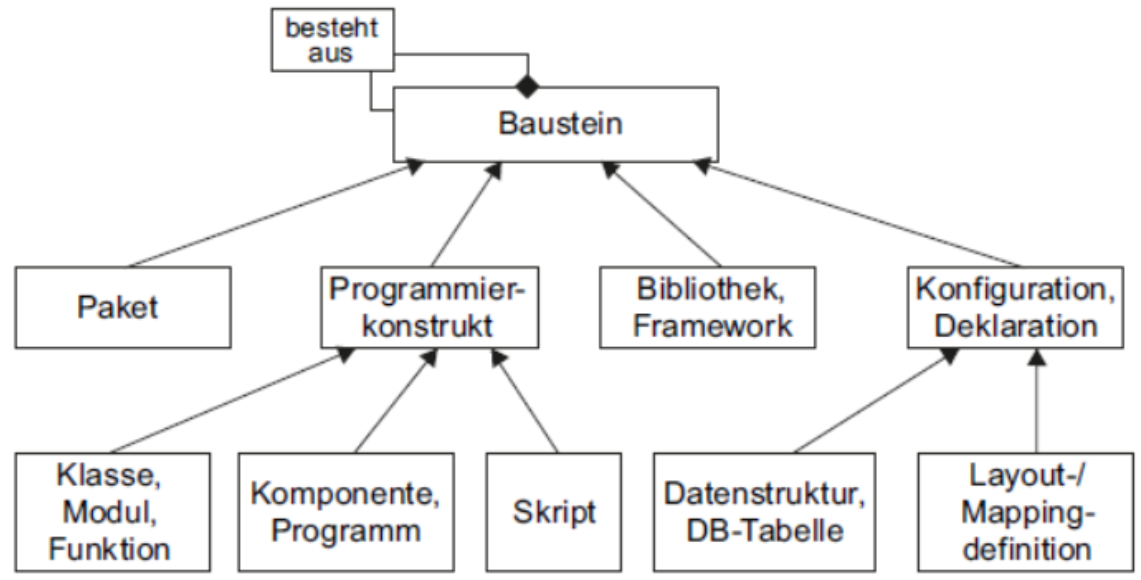
\includegraphics[width=150px]{img/Bausteine.png}
        \captionof{figure}{Abbildung Bausteine}
        \label{fig:Abbildung Bausteine}
\end{Figure}

\begin{itemize}
   \item Bausteine bieten Schnittstelle an, welche er im Sinne eines Vertrags garantiert
   \item Über die angebotene und benötigten Schnittstellen kapselt der Baustein die Implementierung dieser Schnittstelle
   \subitem $\rightarrow$ Dadurch kann er durch einen anderen Baustein ersetzt werden, die dieselben Schnittstellen exportieren und gegebenfalls importieren
   \item Bausteine können auch hierarchische (De-)Kompositionen beinhalten
   \item \textbf{Blackbox-Sicht} man sieht nur die exportierten und importierten Schnittstellen $\rightarrow$ respektiert das Geheimnisprinzip
   \subitem $\Rightarrow$ Sicht des \textbf{Bausteinnutzers} 
   \item \textbf{Greybox-Sicht (auch: Konfiguration)} zeigt wie importierte Schnittstellen mit den exportierten Schnittstellen verschaltet werden
   \subitem $\Rightarrow$ Sicht des \textbf{Bausteinkonfigurators} 
   \item \textbf{Whitebox-Sicht (auch: Glassbox-Sicht)} erlaubt Blick ins innere
   \subitem $\Rightarrow$ Sicht des \textbf{Bausteinimplementierers}  
\end{itemize}

\subsection{Schnittstellen}

\begin{itemize}
   \item Standardschnittstelle
   \subitem Wird von ausserhalb definiert. Sowohl der importierende als auch der exportierende Baustein halten sich daran 
   \item Angebotene Schnittstelle
   \subitem definiert durch den Exporteur, neben Standardschnittstelle die meistverwendete 
   \item Angeforderte Schnittstelle
   \subitem definiert durch den Importeur, häufig bei Frameworks anzutreffen
   \item unabhängige Schnittstelle
   \subitem Importeur und Exporteur hat eigene Schnittstelle, es braucht einen Adapter(-Pattern)  
\end{itemize}

\begin{Figure}
   \centering
    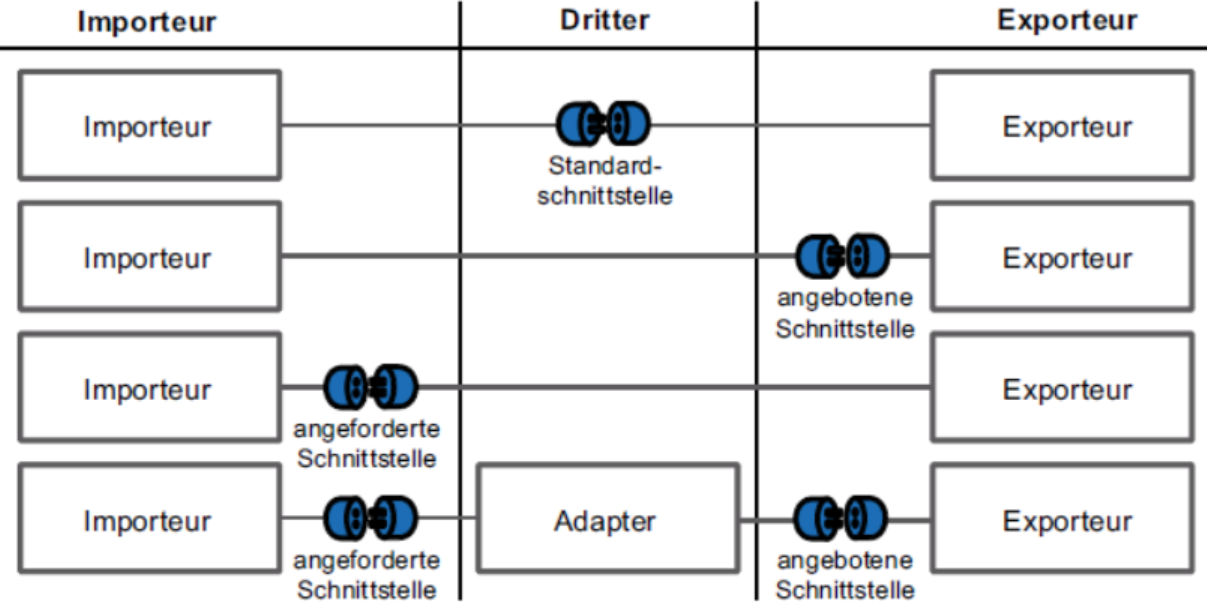
\includegraphics[width=150px]{img/Schnittstellen.png}
        \captionof{figure}{Abbildung Schnittstellenvarianten}
        \label{fig:Abbildung Schnittstellenvarianten}
\end{Figure}

\subsection{Softwarearchitekturbeschreibung}
\begin{itemize}
   \item Dabei wird das System von seiner Umgebung beeinflusst und umgekehrt
   \item Jedes System hat eine Architektur
   \item Die Architektur wird laut Standard durch eine einzige Architekturbeschreibung beschrieben
   \item Darüber hinaus hat ein System eine Reihe von Interessenvertretern (Stakeholder)
   \item Die Stakeholder haben eine Menge von Anliegen
   \item Die Architekturbeschreibung nimmt die Anliegen der Stakeholder auf und begründet damit die getroffenen Architekturentscheidungen in den Begründungen
\end{itemize}

\begin{Figure}
   \centering
    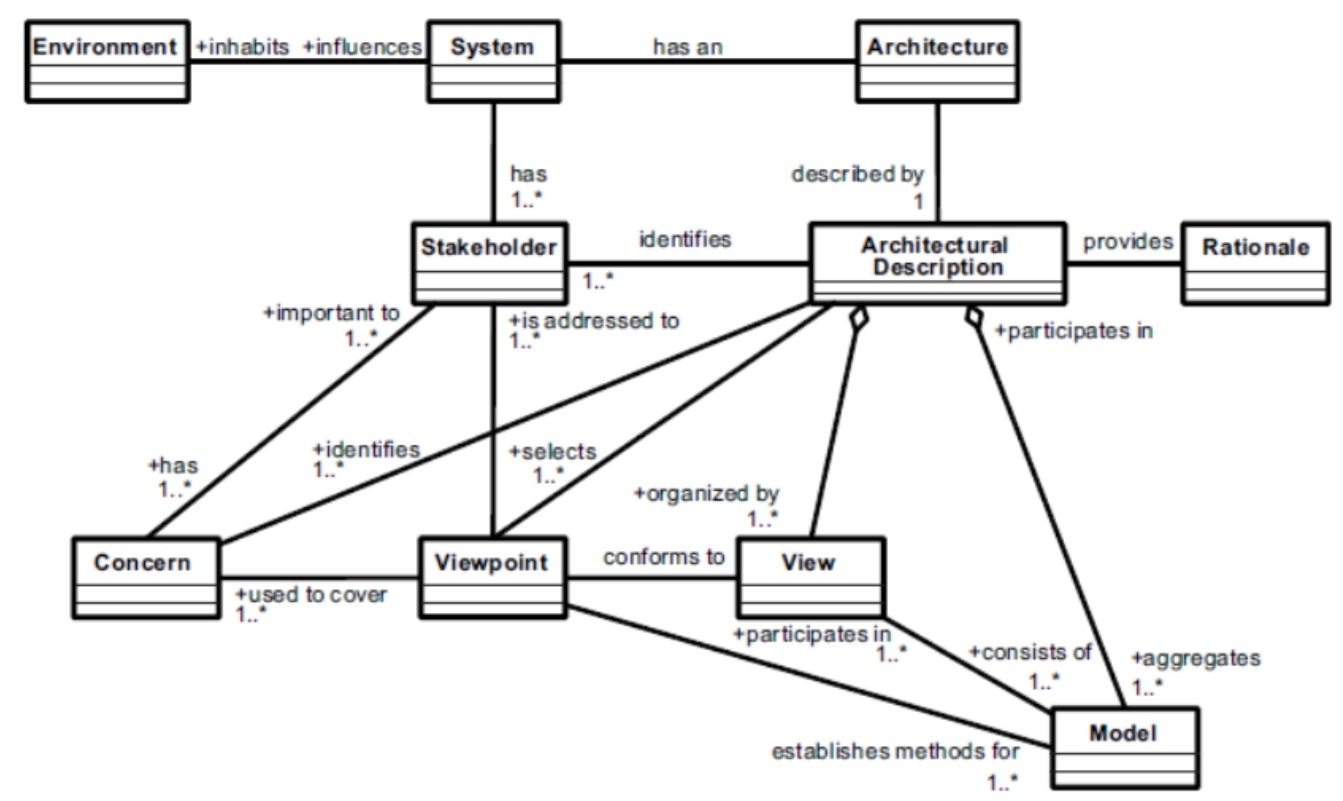
\includegraphics[width=150px]{img/konzModelArch.png}
        \captionof{figure}{Abbildung Kernelemente des konzeptionellen Modells gemaess IEEE-Standard 1471-2000}
        \label{fig:Abbildung Kernelemente des konzeptionellen Modells gemaess IEEE-Standard 1471-2000}
\end{Figure}

\subsubsection{Architektursichten}
Architekturbeschreibungen sind Sichten auf die Architekturbeschreibung\\
nach IEEE gibt es Standard-Sichten:
\begin{itemize}
   \item functional view
   \item physical view 
   \item technical view
\end{itemize}

Diese Sichten sind im Verständnis von Philippe Kruchten \textit{Architectural Blueprints}
\begin{Figure}
   \centering
    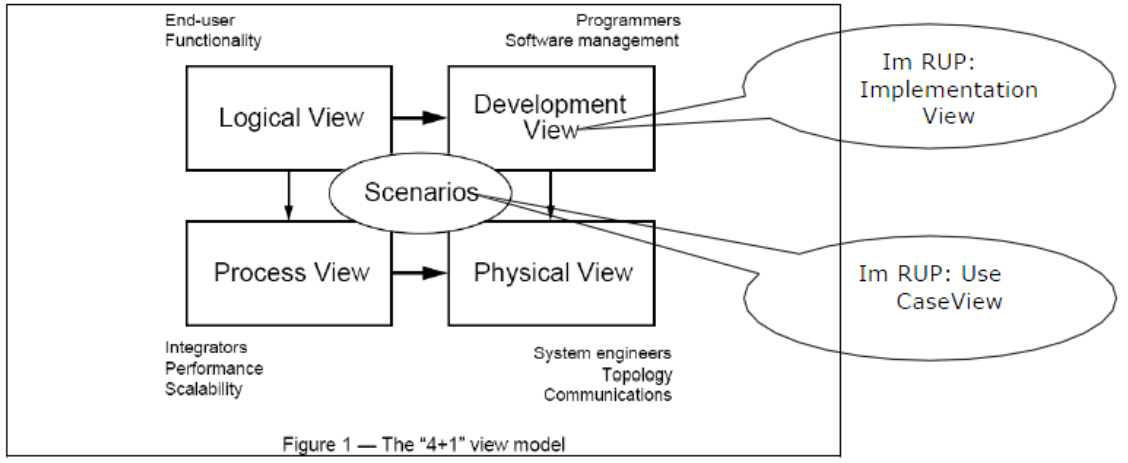
\includegraphics[width=150px]{img/4Plus1.png}
        \captionof{figure}{Abbildung Architectural Blueprints}
        \label{fig:Abbildung Architectural Blueprints}
\end{Figure}

\subsubsection{Architekturebene}
Eine Architekturbeschreibung besteht dabei aus einer Menge von Architekturebenen

\begin{Figure}
   \centering
    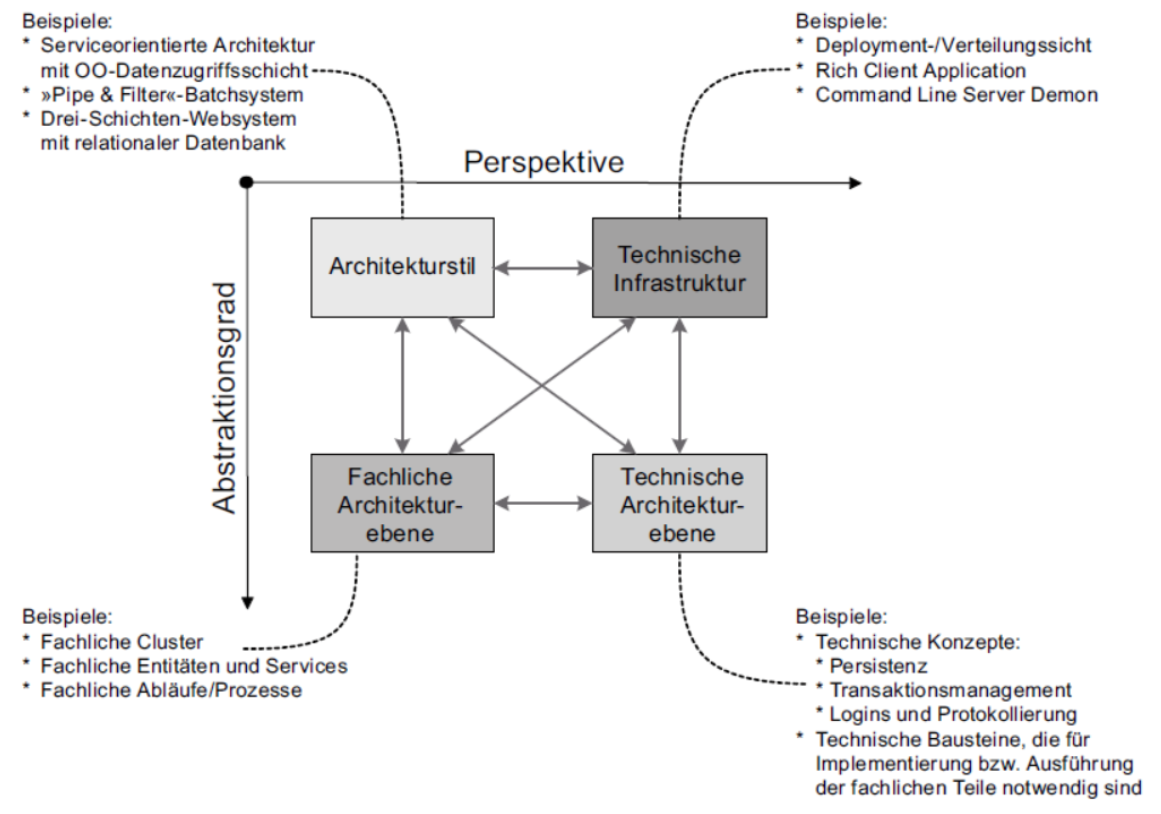
\includegraphics[width=150px]{img/Architekturebene.png}
        \captionof{figure}{Abbildung Architekturebene}
        \label{fig:Abbildung Architekturebene}
\end{Figure}

\begin{itemize}
   \item Architekturebene können für sich alleine betrachtet werden, allerdings beeinfluss sie sich gegeneinander und sind somit voneinander abhängig
   \item Der \textbf{Architekturstil} ist dabei die zentrale Architekturmetapher des Systems 
   \subitem \textit{Drei-Schichten-Architektur unter Verwendung eines Model-View-Controllers in der Präsentationsschicht und einem objektrelationalen Mapping in der Datenhaltungsschicht strukturiert}
   \item \textbf{technische Infrastruktur} hingegen fixiert die Netzwerkschnittstelle der Architektur
   \subitem \textit{Wir haben einen Thin Client mit einem Web- und Application Container und einer relationen DB} 
\end{itemize}

\subsubsection{Wechselwirkung}
\begin{itemize}
   \item Die Architektur wird von der Umgebung beeinflusst und umgekehrt
   \item Folgende Beispiele der Wechselwirkung werden aufgelistet
   \subitem Projektumfeld und Projektmanagement
   \subitem Produktmanagement und RE
   \subitem Ausführungsplattform und Betrieb
   \subitem Werkzeugumgebung und Entwicklung 
\end{itemize}

\begin{Figure}
   \centering
    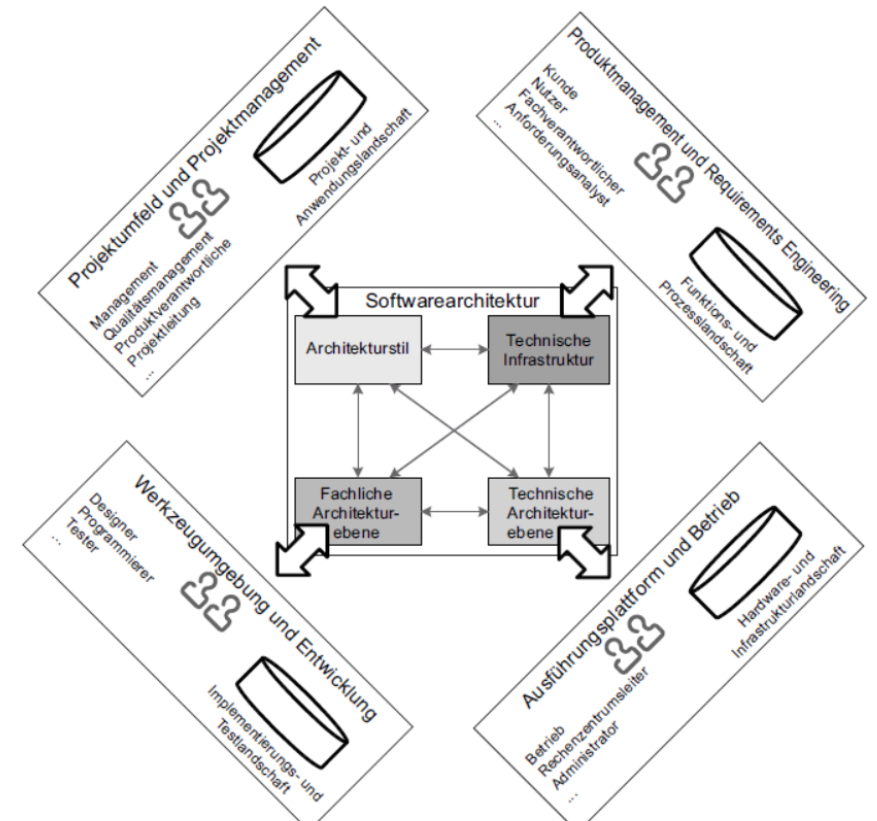
\includegraphics[width=150px]{img/Wechselwirkung.png}
        \captionof{figure}{Abbildung des Gesamtbildes}
        \label{fig:Abbildung des Gesamtbildes}
\end{Figure}

\subsection{Qualität und NUtzen der Softwarearchitektur}
\begin{itemize}
   \item Die Qualität der Softwarearchitektur kann nur im Kontext konkreter Qualitätsziele bewertet werden
   \item Diese Qualitätsziele werden von den Anforderungen, insbesondere von den nichtfunktionalen Anforderungen und geforderten Qualitätseigenschaften abgeleitet und sind somit spezifisch für das konkrete Softwaresystem
   \item Qualitäte lassen sich nur indirekt durch Merkamle beschreiben
\end{itemize}

\subsubsection{Qualitätsmerkmale}
\begin{itemize}
   \item Funktionalität
   \item Zuverlässigkeit
   \item Benutzbarkeit
   \item Effizienz
   \item Änderbarkeit
   \item Übertragbarkeit
\end{itemize}

\subsubsection{Twin Peak Model}
Zeigt die Softwarearchitektur aus der Vogelperspektive

\begin{Figure}
   \centering
    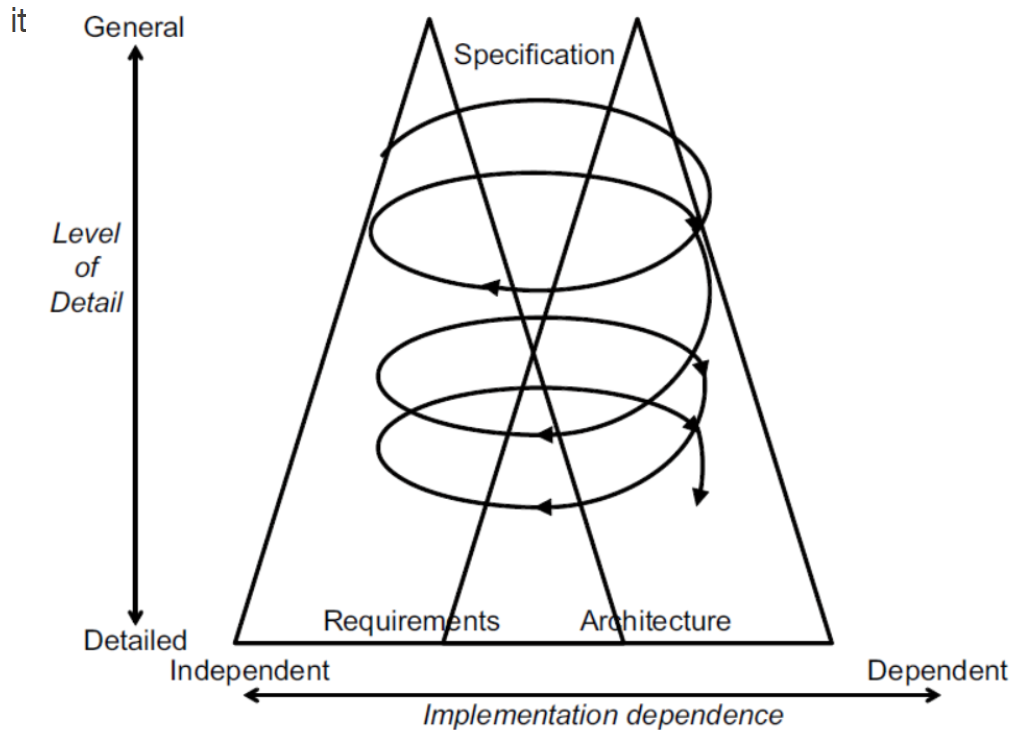
\includegraphics[width=150px]{img/TwinPeakMOdel.png}
        \captionof{figure}{Abbildung der Architektur aus der Vogelperspektive}
        \label{fig:Abbildung der Architektur aus der Vogelperspektive}
\end{Figure}

\subsection{Softwarearchitekturentwurf}

\subsubsection{Architecture Business Cycle}
\begin{Figure}
   \centering
    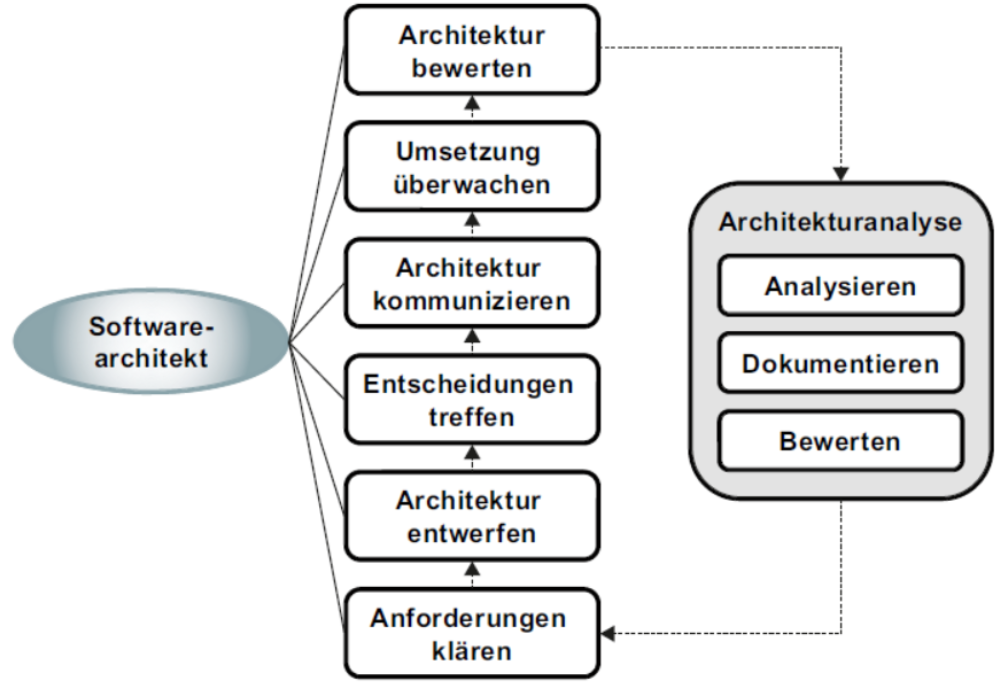
\includegraphics[width=150px]{img/ArchitectureBusinessCycle.png}
        \captionof{figure}{Ablauf des Architecture Business Cycle}
        \label{fig:Ablauf des Architecture Business Cycle}
\end{Figure}


\subsubsection{Alternatives Modell}
\begin{itemize}
   \item Anforderungen und Randbedingungen analyisieren
   \subitem funktionale und nichtfunktionale Anforderungen untersuchen
   \subitem Qualität und Stabilität überprüfen
   \subitem Lücken in Anforderungen aufdekcen
   \subitem erstes Verständnis für den Architekturstil
   \item Architektursichten und technische Konzepte entwerfen
   \subitem Architektur detaillierter ausarbeiten
   \subitem Sichtenbasierte Beschreibung der unterschiedlichen Architekturebene
   \subitem funktionale Anforderungen auf fachliche Architekturebene herunterbrechen
   \item Architektur und Entwurfsentscheidungen bewerten
   \subitem erarbeitete Architektur muss qualitätsgesichert werden
   \subitem konkrete Szenarien erarbeiten
   \item Umsetzung begleiten und überprüfen
   \subitem Kommunizieren von Entwickler bis zum Kunden 
\end{itemize}

\begin{Figure}
   \centering
    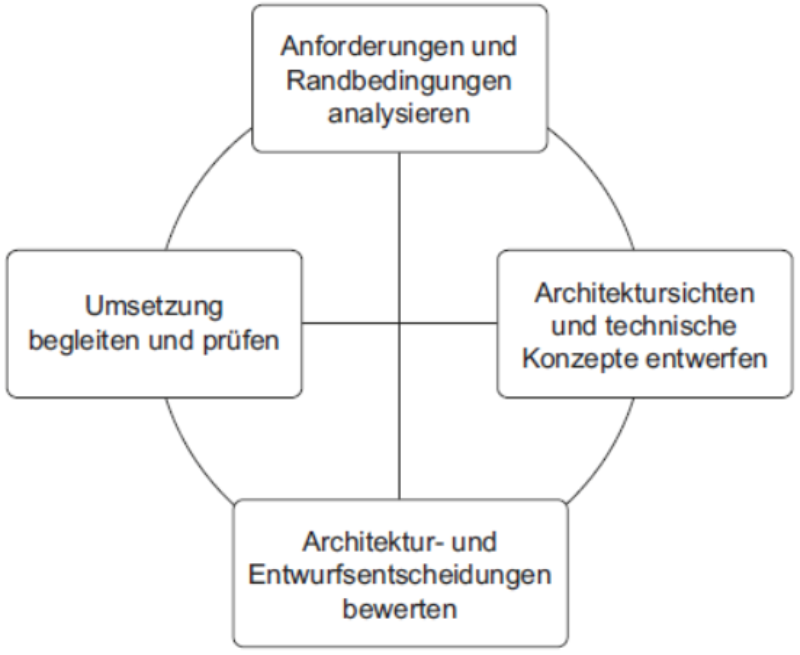
\includegraphics[width=150px]{img/AlternativesModell.png}
        \captionof{figure}{Ablauf des alternativen Modells}
        \label{fig:Ablauf des alternativen Modells}
\end{Figure}

\subsection{Der Softwarearchitekt}
\begin{itemize}
   \item kommuniziert gerne 
   \item Hat Kontakt zu allen anderen Stakeholder
   \item ist verantwortlich, dass das System den sicherheitanforderungen genügeträgt
   \item Machbarkeit der Anforderungen abklärt
   \item Priorisiert die funktionalen und nichtfunktionalen Arbeiten
   \item Zeit Integrationsmöglichkeiten
   \item erarbeitet, evaluiert und bewertet Lösungsansätze
   \item Zentraler Ansprechpartner
   \item Grosse Strukturierung des Systems
   \item Integriert neue Technologien
   \item Verantwortlich der Programmierrichtlinien
   \item unterstützt Tester
   \item erklärt Architektur und gibt Erfahrung an Entwickler weiter
\end{itemize}

\section{Entwurf von Softwarearchitekturen}

\subsection{Entwurfsprinzipien}


\subsection{Architekturzentriere Entwicklungsansätze}


\subsection{Architekturmuster}


\subsection{Entwurfsmuster}

\end{document}